\documentclass[11pt,a4paper]{ctexart}
% Shared preamble for the assignment reports. Use with:
%   \documentclass[11pt,a4paper]{ctexart}  (XeLaTeX)
%   % Shared preamble for the assignment reports. Use with:
%   \documentclass[11pt,a4paper]{ctexart}  (XeLaTeX)
%   % Shared preamble for the assignment reports. Use with:
%   \documentclass[11pt,a4paper]{ctexart}  (XeLaTeX)
%   \input{../common/preamble.tex}
\usepackage[margin=2.3cm]{geometry}
\setmainfont{texgyretermes}[Extension=.otf,UprightFont=*-regular,BoldFont=*-bold,ItalicFont=*-italic,BoldItalicFont=*-bolditalic]
\setsansfont{texgyreheros}[Extension=.otf,UprightFont=*-regular,BoldFont=*-bold,ItalicFont=*-italic,BoldItalicFont=*-bolditalic]
\setmonofont{texgyrecursor}[Extension=.otf,UprightFont=*-regular,BoldFont=*-bold,ItalicFont=*-italic,BoldItalicFont=*-bolditalic]
\usepackage{amsmath,amssymb,mathtools,bm}
\usepackage{graphicx}
\usepackage{booktabs,multirow,makecell,array,tabularx}
\usepackage[table]{xcolor}
\usepackage[most]{tcolorbox}
\usepackage{enumitem}
\usepackage{listings}
\usepackage{subcaption}
\usepackage{siunitx}
\usepackage[hidelinks]{hyperref}
\usepackage[nameinlink,noabbrev]{cleveref}
\usepackage{float}

\setlength{\emergencystretch}{3em}
\linespread{1.15}
\setlist{leftmargin=*,itemsep=2pt,topsep=3pt}
\graphicspath{{figures/}}

\crefname{figure}{图}{图}
\crefname{table}{表}{表}
\crefname{section}{第}{第}
\creflabelformat{section}{#2#1#3 节}
\crefname{equation}{式}{式}
\crefformat{equation}{式~(#2#1#3)}

\lstset{basicstyle=\ttfamily\footnotesize,columns=fullflexible,breaklines=true,frame=single,
  framerule=0.3pt,rulecolor=\color{black!40},backgroundcolor=\color{black!3},
  keywordstyle=\color{blue!60!black}\bfseries,commentstyle=\color{green!40!black},
  numbers=left,numberstyle=\tiny\color{black!50},xleftmargin=1.5em}

% Interview boxes: question, model answer, common wrong answer.
\newtcolorbox{iqbox}[1]{enhanced,breakable,colback=blue!3,colframe=blue!45!black,boxrule=0.5pt,arc=1.5pt,
  left=4pt,right=4pt,top=3pt,bottom=3pt,fonttitle=\bfseries\small,title={面试追问：#1}}
\newtcolorbox{findingbox}[1][]{enhanced,breakable,colback=green!3,colframe=green!40!black,boxrule=0.5pt,arc=1.5pt,
  left=4pt,right=4pt,top=3pt,bottom=3pt,fonttitle=\bfseries\small,title={结论#1}}
\newtcolorbox{caveatbox}{enhanced,breakable,colback=orange!4,colframe=orange!60!black,boxrule=0.5pt,arc=1.5pt,
  left=4pt,right=4pt,top=3pt,bottom=3pt,fonttitle=\bfseries\small,title={不能推出的结论}}

\newcommand{\authorline}{ShaneLiu04\thanks{GitHub: \url{https://github.com/ShaneLiu04}。代码与原始指标：\url{https://gitee.com/liu-xingyan04/mlsys-infra}。本文基于公开课程材料独立完成，与课程团队无隶属关系。}}

\usepackage[margin=2.3cm]{geometry}
\setmainfont{texgyretermes}[Extension=.otf,UprightFont=*-regular,BoldFont=*-bold,ItalicFont=*-italic,BoldItalicFont=*-bolditalic]
\setsansfont{texgyreheros}[Extension=.otf,UprightFont=*-regular,BoldFont=*-bold,ItalicFont=*-italic,BoldItalicFont=*-bolditalic]
\setmonofont{texgyrecursor}[Extension=.otf,UprightFont=*-regular,BoldFont=*-bold,ItalicFont=*-italic,BoldItalicFont=*-bolditalic]
\usepackage{amsmath,amssymb,mathtools,bm}
\usepackage{graphicx}
\usepackage{booktabs,multirow,makecell,array,tabularx}
\usepackage[table]{xcolor}
\usepackage[most]{tcolorbox}
\usepackage{enumitem}
\usepackage{listings}
\usepackage{subcaption}
\usepackage{siunitx}
\usepackage[hidelinks]{hyperref}
\usepackage[nameinlink,noabbrev]{cleveref}
\usepackage{float}

\setlength{\emergencystretch}{3em}
\linespread{1.15}
\setlist{leftmargin=*,itemsep=2pt,topsep=3pt}
\graphicspath{{figures/}}

\crefname{figure}{图}{图}
\crefname{table}{表}{表}
\crefname{section}{第}{第}
\creflabelformat{section}{#2#1#3 节}
\crefname{equation}{式}{式}
\crefformat{equation}{式~(#2#1#3)}

\lstset{basicstyle=\ttfamily\footnotesize,columns=fullflexible,breaklines=true,frame=single,
  framerule=0.3pt,rulecolor=\color{black!40},backgroundcolor=\color{black!3},
  keywordstyle=\color{blue!60!black}\bfseries,commentstyle=\color{green!40!black},
  numbers=left,numberstyle=\tiny\color{black!50},xleftmargin=1.5em}

% Interview boxes: question, model answer, common wrong answer.
\newtcolorbox{iqbox}[1]{enhanced,breakable,colback=blue!3,colframe=blue!45!black,boxrule=0.5pt,arc=1.5pt,
  left=4pt,right=4pt,top=3pt,bottom=3pt,fonttitle=\bfseries\small,title={面试追问：#1}}
\newtcolorbox{findingbox}[1][]{enhanced,breakable,colback=green!3,colframe=green!40!black,boxrule=0.5pt,arc=1.5pt,
  left=4pt,right=4pt,top=3pt,bottom=3pt,fonttitle=\bfseries\small,title={结论#1}}
\newtcolorbox{caveatbox}{enhanced,breakable,colback=orange!4,colframe=orange!60!black,boxrule=0.5pt,arc=1.5pt,
  left=4pt,right=4pt,top=3pt,bottom=3pt,fonttitle=\bfseries\small,title={不能推出的结论}}

\newcommand{\authorline}{ShaneLiu04\thanks{GitHub: \url{https://github.com/ShaneLiu04}。代码与原始指标：\url{https://gitee.com/liu-xingyan04/mlsys-infra}。本文基于公开课程材料独立完成，与课程团队无隶属关系。}}

\usepackage[margin=2.3cm]{geometry}
\setmainfont{texgyretermes}[Extension=.otf,UprightFont=*-regular,BoldFont=*-bold,ItalicFont=*-italic,BoldItalicFont=*-bolditalic]
\setsansfont{texgyreheros}[Extension=.otf,UprightFont=*-regular,BoldFont=*-bold,ItalicFont=*-italic,BoldItalicFont=*-bolditalic]
\setmonofont{texgyrecursor}[Extension=.otf,UprightFont=*-regular,BoldFont=*-bold,ItalicFont=*-italic,BoldItalicFont=*-bolditalic]
\usepackage{amsmath,amssymb,mathtools,bm}
\usepackage{graphicx}
\usepackage{booktabs,multirow,makecell,array,tabularx}
\usepackage[table]{xcolor}
\usepackage[most]{tcolorbox}
\usepackage{enumitem}
\usepackage{listings}
\usepackage{subcaption}
\usepackage{siunitx}
\usepackage[hidelinks]{hyperref}
\usepackage[nameinlink,noabbrev]{cleveref}
\usepackage{float}

\setlength{\emergencystretch}{3em}
\linespread{1.15}
\setlist{leftmargin=*,itemsep=2pt,topsep=3pt}
\graphicspath{{figures/}}

\crefname{figure}{图}{图}
\crefname{table}{表}{表}
\crefname{section}{第}{第}
\creflabelformat{section}{#2#1#3 节}
\crefname{equation}{式}{式}
\crefformat{equation}{式~(#2#1#3)}

\lstset{basicstyle=\ttfamily\footnotesize,columns=fullflexible,breaklines=true,frame=single,
  framerule=0.3pt,rulecolor=\color{black!40},backgroundcolor=\color{black!3},
  keywordstyle=\color{blue!60!black}\bfseries,commentstyle=\color{green!40!black},
  numbers=left,numberstyle=\tiny\color{black!50},xleftmargin=1.5em}

% Interview boxes: question, model answer, common wrong answer.
\newtcolorbox{iqbox}[1]{enhanced,breakable,colback=blue!3,colframe=blue!45!black,boxrule=0.5pt,arc=1.5pt,
  left=4pt,right=4pt,top=3pt,bottom=3pt,fonttitle=\bfseries\small,title={面试追问：#1}}
\newtcolorbox{findingbox}[1][]{enhanced,breakable,colback=green!3,colframe=green!40!black,boxrule=0.5pt,arc=1.5pt,
  left=4pt,right=4pt,top=3pt,bottom=3pt,fonttitle=\bfseries\small,title={结论#1}}
\newtcolorbox{caveatbox}{enhanced,breakable,colback=orange!4,colframe=orange!60!black,boxrule=0.5pt,arc=1.5pt,
  left=4pt,right=4pt,top=3pt,bottom=3pt,fonttitle=\bfseries\small,title={不能推出的结论}}

\newcommand{\authorline}{ShaneLiu04\thanks{GitHub: \url{https://github.com/ShaneLiu04}。代码与原始指标：\url{https://gitee.com/liu-xingyan04/mlsys-infra}。本文基于公开课程材料独立完成，与课程团队无隶属关系。}}

\graphicspath{{../../solutions/cs149/asst3-scan-render/artifacts/figures/}}

\title{CS149 Assignment 3 复刻报告：\\CUDA 上的 SAXPY、并行前缀和与保序圆渲染器}
\author{\authorline}
\date{2026 年 10 月}

\begin{document}
\maketitle

\begin{abstract}
本文复刻 Stanford CS149（Fall 2024）Assignment 3「A Simple Renderer in CUDA」的三个部分，并保留本实验目录原有的 numpy 版
（work/span 计数、乱序误差、tile 分桶测试次数）作为算法层面的对照。GPU 部分全部用 CUDA C++ 手写，在 RTX 5090（sm\_120，
170 SM，96 MB L2，GDDR7 标称 1.79 TB/s，PCIe 5.0 x16）上测量：
(1) SAXPY 在 $N=2^{28}$ 时 kernel 达到 1578 GB/s（标称带宽的 88\%），而包含 \texttt{cudaMemcpy} 的端到端只有 53.8 GB/s（pinned）
和 10.5 GB/s（pageable），kernel 只占端到端时间的 3.4\%；4 个 stream 分块流水把 H2D 与 D2H 重叠后达到 77.1 GB/s。
(2) 六种 exclusive scan 在 $10^3$–$2^{28}$、含非 2 的幂长度下全部与 CPU 逐元素一致。starter 结构的 global-memory Blelloch 每层一次 launch，
$2^{28}$ 时 16.75 ms；shared-memory 块内 scan + 递归块和 2.82 ms；\texttt{cub::DeviceScan} 1.41 ms。三者换算到实际 DRAM 流量后都在
约 1.52 TB/s，差距来自访存次数（$\approx 84N$、$16N$、$8N$ 字节），不是算力。小 $N$ 时时间由 launch 数决定：$N=1000$ 时 naive 20 次 launch 用 49.6\,$\mu$s，
单 block 版 4.4\,$\mu$s。基于 scan 的 \texttt{find\_repeats} 在 $10^8$ 时 1.87 ms，比 \texttt{thrust::copy\_if}（0.28 ms）慢 6.6 倍，原因同样是多遍访存。
(3) 渲染器在 9 个 $1024\times1024$ 场景上，starter 式「一线程一圆」kernel 在除 rgb 外的 8 个场景中 48.5\%–100\% 像素出错（rgb 为 24.3\%），且多数场景两次运行结果不同；
四个正确版本对 90 个（场景, 阶段, tile）组合的最大绝对误差为 0（snow 场景为 $2.98\times10^{-7}$，来自 \texttt{expf}）。
用 scan 做全局分桶并在 shared memory 中批量取圆后，rand1M 从「每像素遍历所有圆」的 844 ms 降到 0.538 ms，比单核 CPU 顺序参考快 712 倍。
tile 大小的最优值随圆半径变化：小圆场景 $T=8$，其余多为 $T=16$。
\end{abstract}

\tableofcontents
\newpage

%=====================================================================
\section{背景与作业要求}

CS149~\cite{cs149} Assignment 3 的官方 starter 是 CUDA 代码，包含三部分。本目录（\path{solutions/cs149/asst3-scan-render}）原先只有 numpy 版，
本次补上 GPU 部分。对应关系见\cref{tab:map}。

\begin{table}[H]
\centering\small
\caption{官方作业部分与本仓库实现的对应}\label{tab:map}
\begin{tabularx}{\linewidth}{p{3.0cm}XX}
\toprule
官方部分 & 本仓库 CPU/numpy 实现（已有） & 本次 GPU 实现（\texttt{gpu/}） \\
\midrule
Part 1 SAXPY & 无（见 asst1 prog5） & \texttt{saxpy.cu}：kernel 带宽 vs $N$；端到端 pinned / pageable / 4-stream 分块流水；launch 开销 \\
Part 2 \texttt{exclusive\_scan} & \texttt{scan.py}：顺序、Hillis~\cite{hillis1986}--Steele、Blelloch~\cite{blelloch1990}，work/span 计数 & \texttt{scan.cu}：naive（starter 结构，每层一次 launch）、shared-memory Blelloch（有/无 bank padding）、raking + warp shuffle、thrust、cub \\
Part 2 \texttt{find\_repeats} & \texttt{primitives.py}：flags $\to$ scan $\to$ scatter & flag kernel $\to$ 自写 scan $\to$ scatter，对比 \texttt{thrust::copy\_if} \\
Part 3 circle renderer & \texttt{renderer.py}：顺序参考、乱序模拟、tile 分桶~\cite{laine2011} + scan 压缩~\cite{sengupta2007} & \texttt{render.cu}：CPU 顺序参考、naive 一线程一圆（错误）、每像素全圆、全局 scan 分桶、分桶 + shared 批量、块内 scan 分桶 \\
\bottomrule
\end{tabularx}
\end{table}

\paragraph{渲染器的两个正确性约束。} 官方文档要求：(1) \emph{原子性}：对同一像素的「读--混合~\cite{porter1984}--写」不能被其他圆的更新打断；
(2) \emph{顺序}：同一像素上的圆必须按输入顺序混合。混合公式是 over 算子
\begin{equation}
\mathbf{c} \leftarrow \alpha\,\mathbf{rgb}_k + (1-\alpha)\,\mathbf{c},\label{eq:over}
\end{equation}
两个圆交换顺序，结果不同（不满足交换律），所以「按圆并行 + 原子操作」也不够，必须保序。starter 给出的 \texttt{kernelRenderCircles}
一线程处理一个圆，两个约束都违反。作业的核心是把并行轴从「圆」换到「像素/tile」，并用 scan 在不做全局排序的前提下，为每个 tile 生成有序的圆列表。

%=====================================================================
\section{实验环境}

\begin{table}[H]
\centering\small
\caption{实验环境}\label{tab:env}
\begin{tabularx}{\linewidth}{lX}
\toprule
GPU & NVIDIA GeForce RTX 5090，32 GB（32607 MiB），170 SM，sm\_120（Blackwell），L2 100663296 B（96 MB），每 SM 共享内存 102400 B，每 SM 最多 1536 线程；
驱动 595.71.05；PCIe 链路 Gen5 x16（\texttt{nvidia-smi} 读到 current = max = 5，width 16）\\
GPU 带宽参考 & GDDR7 标称 1.79 TB/s（28 Gbps $\times$ 512 bit）；同机 asst1 已测 SAXPY kernel $\approx$1.55 TB/s、端到端 $\approx$52 GB/s；PCIe 5.0 x16 单向标称 64 GB/s\\
主机 CPU & 2 路 Intel Xeon Gold 6459C（容器可见 128 逻辑核，cgroup 限 16 核，本实验只用 \texttt{taskset -c 33,34}）；CPU 参考渲染器为单线程\\
工具链 & CUDA 12.8 \texttt{nvcc -O3 -arch=sm\_120 -std=c++17}；g++ 11.4；thrust/cub 随 CUDA 12.8；\texttt{render} 额外加 \texttt{-fmad=false}，使 device 端算术与 host 参考逐位一致\\
计时 & \texttt{cudaEvent}，预热 2--3 次后取 5--50 次的中位数；端到端用 \texttt{steady\_clock} + 同步；所有 GPU 任务都在 \texttt{flock /root/autodl-tmp/gpu.lock} 下独占运行\\
分析器 & \texttt{ncu} 报 \texttt{ERR\_NVGPUCTRPERM}（容器内无性能计数器权限，见 \texttt{ncu\_attempt.txt}），改用 \texttt{cudaFuncGetAttributes} + 占用率 API 获得寄存器数与理论 occupancy\\
本地 & Windows Server，4 物理核；Python 3.12、numpy、matplotlib；numpy 版实验与全部绘图在本地运行\\
\bottomrule
\end{tabularx}
\end{table}

原始数据在 \path{artifacts/raw/gpu/} 下：\texttt{saxpy}、\texttt{scan}、\texttt{find\_repeats}、\texttt{render}、\texttt{render\_sweep}、
\texttt{render\_attrs}、\texttt{scan\_attrs} 七个 \texttt{.jsonl} 文件；图像在 \path{artifacts/raw/gpu/images/}（参考图与 naive 图为 512 像素缩略 PNG，差值图为 $1024^2$ 全分辨率 8-bit）。
复现命令：
\begin{lstlisting}[language=bash,numbers=none]
bash gpu/build.sh && bash gpu/run_gpu.sh all && python scripts/plot_gpu.py
\end{lstlisting}

%=====================================================================
\section{方法与实现}

\subsection{Part 1：SAXPY 与传输开销}
kernel 为一线程一元素 \texttt{y[i] = a*x[i] + y[i]}，256 线程/块。每个 $N=2^{10},2^{12},\dots,2^{28}$ 测四个量：
(a) kernel-only（数据已在显存）；(b) pinned：\texttt{cudaMallocHost} 内存上 H2D($x,y$) + kernel + D2H($y$)；
(c) pageable：同样流程，主机内存是 \texttt{std::vector}；(d) streams：pinned 内存切 16 块轮流放进 4 个 stream，
H2D、kernel、D2H 异步排队，使不同块的上行和下行拷贝重叠。四者都按 $12N$ 字节（读 $x$、读 $y$、写 $y$）折算有效带宽。
另测空 kernel 连续 launch 的平均间隔，以及 launch 加同步的往返时间。

\subsection{Part 2：六种 exclusive scan}

\paragraph{naive（starter 结构）。} 输入复制到长度 $m=2^{\lceil\log_2 N\rceil}$ 的缓冲区，尾部补 0；up-sweep 每层一次 launch，
根置 0，down-sweep 每层一次 launch，共 $2\log_2 m$ 次 launch（测试 \path{test_naive_scan_launches_are_2log2m} 逐行检查）。

\begin{lstlisting}[language=C++,caption={starter 结构的 up-sweep / down-sweep kernel（\texttt{scan.cu}）}]
__global__ void upsweep_k(int* a, long long m, long long two_d) {
  long long i = (long long)(blockIdx.x * (long long)blockDim.x + threadIdx.x) * 2 * two_d;
  if (i < m) a[i + 2 * two_d - 1] += a[i + two_d - 1];
}
__global__ void downsweep_k(int* a, long long m, long long two_d) {
  long long i = ...same...;
  if (i < m) { int t = a[i + two_d - 1];
               a[i + two_d - 1] = a[i + 2 * two_d - 1];
               a[i + 2 * two_d - 1] += t; }
}
\end{lstlisting}

\paragraph{smem / smem\_nopad。} 采用 GPU Gems 3 第 39 章的做法\cite{harris2007}：每块 512 线程处理 1024 个元素，在 shared memory 中做
Blelloch up/down-sweep。块总和写入 \texttt{sums[]}，对 \texttt{sums} 递归调用同一过程，最后用 \texttt{uniform\_add} 把块前缀加回去。
padding 版每 32 个元素插 1 个空位（\texttt{CF(i) = i>>5}），用来消除深层 stride 访问的 bank conflict。

\begin{lstlisting}[language=C++,caption={块内 Blelloch（节选）与递归驱动}]
for (int d = SE >> 1; d > 0; d >>= 1) {          // up-sweep in shared memory
  __syncthreads();
  if (t < d) { int a = off*(2*t+1)-1, b = off*(2*t+2)-1;
               if (PAD) a += CF(a), b += CF(b);
               s[b] += s[a]; }
  off <<= 1;
}
if (t == 0) { if (sums) sums[blockIdx.x] = s[last]; s[last] = 0; }
... down-sweep symmetric ...
void Rec::run(const int* in, int* out, long long n, size_t lvl) {
  unsigned nb = (n + per_block - 1) / per_block;
  if (nb == 1) { block(in, out, nullptr, n, 1); return; }
  block(in, out, lvl_sums[lvl], n, nb);           // pass 1: read N, write N
  run(lvl_sums[lvl], lvl_scan[lvl], nb, lvl + 1); // N/1024 elements
  uniform_add<<<nb, 256>>>(out, lvl_scan[lvl], n, per_block); // pass 2: read N, write N
}
\end{lstlisting}

\paragraph{raking。} 每块 256 线程处理 4096 个元素：先合并访问装入 shared memory（同样 padding），每线程在寄存器里顺序扫 16 个元素，
再用 \texttt{\_\_shfl\_up\_sync} 做 warp 内 inclusive scan，第 0 个 warp 扫 8 个 warp 和。递归结构与 smem 相同，但每块元素数是 4 倍，递归层数和 block 数更少。

\paragraph{thrust / cub。} \texttt{thrust::exclusive\_scan(thrust::device, \dots)} 每次调用内部临时分配缓冲区；
\texttt{cub::DeviceScan::ExclusiveSum} 使用预分配的临时空间。两者底层都是 Merrill--Garland 的单遍 decoupled look-back scan\cite{merrill2016}：
每个元素只读一次、写一次。

\paragraph{测试数据与正确性。} 输入为 \texttt{hash32(i) \& 7}，保证 $2^{28}$ 个元素的总和小于 $2^{31}$；每个 $(N,\text{算法})$ 都把整个输出拷回，
与 CPU 顺序 scan 逐元素比较，mismatch 数写入 \texttt{scan.jsonl}。$N$ 取 19 个值：$10^3$、$2^{10}$、$4096$、$10^4$、$2^{16}$、$10^5$、$2^{18}$、$2^{20}$、
$2^{20}+1$、$10^6$、$3000007$、$2^{22}$、$10^7$、$2^{24}-1$、$2^{24}$、$2^{26}$、$10^8$、$2^{27}$、$2^{28}$。

\paragraph{find\_repeats。} 自写版本为三步：\texttt{repeat\_flags}（\texttt{f[i] = a[i]==a[i+1]}）$\to$ 自写 scan（smem 或 raking）$\to$
\texttt{repeat\_scatter}（scatter 时重新计算谓词，避免再读一遍 flags）；输出个数取 \texttt{pos[n-1]}（因为 \texttt{f[n-1]=0}），需要一次 4 字节 D2H。
对照为 \texttt{thrust::copy\_if(counting\_iterator, \dots, IsRepeat\{a\})}。取值范围为 $[0,100)$ 和 $[0,2)$，对应约 1\% 和 50\% 的重复率。

\subsection{Part 3：渲染器}

\paragraph{场景。} 图像 $1024\times1024$，背景为白色，坐标归一化到 $[0,1]$。所有场景由固定种子的 xorshift 生成，见\cref{tab:scenes}。
\texttt{mean\_coverage} 为 $\sum_k \pi r_k^2$，即平均每个像素被多少个圆覆盖（overdraw）。snow 场景按 $z$ 从远到近排序，颜色和 $\alpha$ 随到圆心的归一化距离衰减：
$\alpha = 0.5\,\mathrm{clamp}(0.6+0.4(1-z))\,e^{-4d^2}$。其他场景 $\alpha=0.5$，与官方 starter 一致。

\begin{table}[H]
\centering\small
\caption{场景定义（\texttt{render.cu: make\_scene}）}\label{tab:scenes}
\begin{tabular}{lrrl}
\toprule
场景 & $N$ & 平均覆盖 & 说明 \\
\midrule
rgb & 3 & 0.8 & 三个大圆（$r=0.3$）互相重叠 \\
rand10k & 10000 & 44.9 & $r\sim U(0.01,0.06)$ \\
rand100k & 100000 & 112.6 & $r\sim U(0.005,0.03)$ \\
biglittle & 50020 & 10.4 & 20 个大圆（$r\in[0.15,0.35]$）在底层，5 万个小圆在上层 \\
littlebig & 50020 & 10.7 & 同上，顺序相反：大圆在最上层 \\
pattern & 5120 & 1.9 & $32^2$ 与 $64^2$ 两层规则网格，半径按正弦变化 \\
snowsingle & 50000 & 39.2 & 雪花着色（径向 $\alpha$ 衰减、\texttt{sqrtf/expf}），按深度排序 \\
rand1M & 1000000 & 59.7 & $r\sim U(0.001,0.007)$ \\
micro2M & 2000000 & 6.8 & $r\sim U(0.0005,0.0015)$，半径约 0.5--1.5 像素 \\
sweep\_$N$ & $10^3$--$3\times10^6$ & $\approx$45 & rand10k 的半径乘 $\sqrt{10^4/N}$，overdraw 保持不变 \\
\bottomrule
\end{tabular}
\end{table}

\paragraph{CPU 参考。} 按输入顺序遍历圆，对每个圆的保守包围盒（\texttt{floor((cx-r)W)} 到 \texttt{ceil((cx+r)W)}）内的像素中心做
\texttt{d2 <= r*r} 测试并按\cref{eq:over}混合。像素中心为 $((x+0.5)/W,(y+0.5)/H)$。host 和 device 共用同一个 \texttt{\_\_host\_\_ \_\_device\_\_ shade()}，
并用 \texttt{-fmad=false} 禁止 FMA 收缩，所以 $\alpha=0.5$ 的场景可以要求 GPU 与 CPU 逐位相等。

\paragraph{五个 GPU 阶段。}
\begin{enumerate}
\item \textbf{naive\_per\_circle}：starter 的 \texttt{kernelRenderCircles}，一线程一圆，对包围盒内像素做非原子的「读--shade--写」。
\item \textbf{allcircles}：一线程一像素（$16\times16$ 块），像素颜色放在寄存器里，按顺序遍历全部 $N$ 个圆，最后写一次。正确，但工作量为 $O(NP)$。
\item \textbf{binned}：全局分桶。\texttt{k\_bin\_count} 计算每个圆覆盖的 tile 数 \texttt{cnt[k]}，并用 \texttt{atomicAdd} 累加每 tile 计数；
对 \texttt{cnt} 做 exclusive scan 得到每个圆的写入偏移；对 tile 计数做 exclusive scan 得到每个 tile 列表的起点 \texttt{tile\_start}；
\texttt{k\_bin\_emit} 按偏移写出 (tile, circle) 对，此时数组按圆的下标排列；最后用 \texttt{cub::DeviceRadixSort::SortPairs} 只对 $\lceil\log_2(\#\text{tiles})\rceil$ 位 key 排序。
radix sort 是稳定的，所以同一 tile 内的圆仍按输入顺序排列。渲染时一个 block 对应一个 tile，每个线程负责一个像素，从 global memory 逐个读取圆参数。
\item \textbf{binned\_smem}：列表与 binned 相同。block 每次协作把 \texttt{blockDim} 个圆的 7 个参数（SoA 布局）装进 shared memory，
同步后每个像素遍历这一批圆（所有线程读同一地址，是 broadcast，没有 bank conflict）。
\item \textbf{blockscan\_smem}：不生成全局列表，是 CS149 常见的参考解法。每个 block 每轮取 \texttt{blockDim} 个圆，每个线程测试一个圆的包围盒是否与本 tile 相交，
对命中标志做 block 级 exclusive scan，得到压缩后的位置，命中的圆按原顺序写入 shared memory，然后所有像素着色这一批圆。整个过程只有一次 launch，但每个 tile 都要测试全部 $N$ 个圆。
\end{enumerate}

\begin{lstlisting}[language=C++,caption={块内 scan 分桶（\texttt{k\_render\_blockscan}，节选）}]
for (int cb = 0; cb < s.n; cb += bs) {
  int k = cb + tid, hit = 0;
  if (k < s.n) { int x0, x1, y0, y1;
    circ_bbox(s.x[k], s.y[k], s.r[k], W, H, x0, x1, y0, y1);
    hit = x0 <= tx1 && x1 >= tx0 && y0 <= ty1 && y1 >= ty0; }
  int total, pos = block_excl_scan(hit, ws, total);  // warp shuffle + warp sums
  if (hit) b.put(pos, s, k);       // compacted, still in input order
  __syncthreads();
  for (int i = 0; i < total; ++i)
    shade(b.x[i], b.y[i], b.z[i], b.r[i], b.R[i], b.G[i], b.B[i], s.snow, fx, fy, c);
  __syncthreads();
}
\end{lstlisting}

\begin{lstlisting}[language=C++,caption={全局分桶的主机端流程（\texttt{Binner::build}，节选）}]
k_bin_count<<<...>>>(s, W, H, T, TX, cnt, tcnt);          // per-circle tile count + per-tile atomics
cub::DeviceScan::ExclusiveSum(tmp, b, cnt, off, s.n);      // circle -> pair offset
cub::DeviceScan::ExclusiveSum(tmp, b, tcnt, tstart, nt+1); // tile -> list start
cudaMemcpy(&last, off + s.n - 1, ...);                     // total pairs (sync)
k_bin_emit<<<...>>>(s, W, H, T, TX, off, k1, v1);          // (tile, circle) in circle order
cub::DeviceRadixSort::SortPairs(tmp, b, k1, k2, v1, v2, pairs, 0, bits); // stable
\end{lstlisting}

\paragraph{计时口径。} 每帧时间包含清屏 kernel。binned 系列包含完整分桶流程（2 次 scan、1 次排序、2 次 4 字节 D2H 同步），
另外单独记录 \texttt{bin\_ms} 和 \texttt{render\_ms}。正确性检查对每个 (场景, 阶段, tile) 都把整帧拷回，与 CPU 参考比较最大绝对误差，
并统计误差 $>10^{-6}$ 和 $>10^{-3}$ 的像素数。naive 阶段额外连续运行两次并统计两次结果不同的像素数。

%=====================================================================
\section{实验结果}

\subsection{CPU/numpy 部分（已有实验回顾）}

这三张图来自原有的 \texttt{scripts/run\_experiments.py}，数据在 \texttt{artifacts/raw/*.csv}。它们给出与硬件无关的计数，GPU 部分的结果要对照这些计数来读。

\begin{figure}[H]\centering
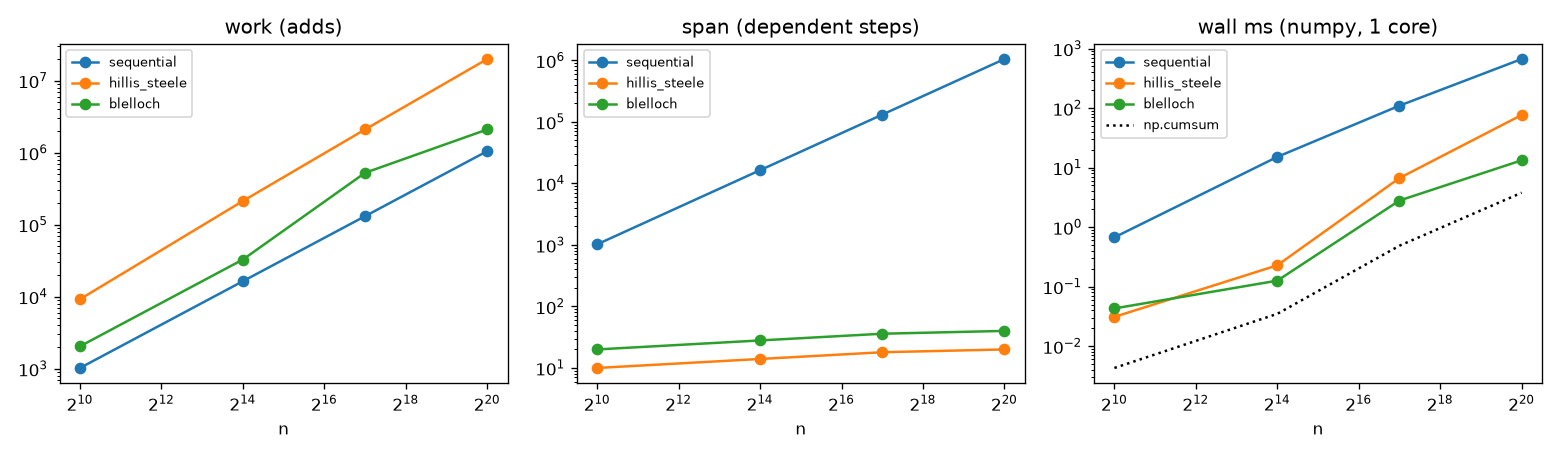
\includegraphics[width=\linewidth]{scan_work_span.png}
\caption{numpy 版 scan 的 work（加法次数）、span（相互依赖的步数）和单核墙钟时间。}\label{fig:cpu-scan}
\end{figure}
\Cref{fig:cpu-scan}：Blelloch 的 work 恒为 $2(m-1)$，Hillis--Steele 为 $\Theta(n\log n)$。$n=2^{20}$ 时两者的加法次数分别为 2.10M 和 19.9M，
单核 numpy 墙钟分别为 13.2 ms 和 76.5 ms。$n=2^{17}+1$ 补齐到 $2^{18}$ 后，Blelloch 的 adds/$n$ 从 2 变成 4。
这对应 GPU 上 naive 版本的补齐代价（\cref{fig:nonpow2}）。span 一列说明 naive GPU 版需要 $2\log_2 m$ 次全局同步，每次同步就是一次 kernel launch。

\begin{figure}[H]\centering
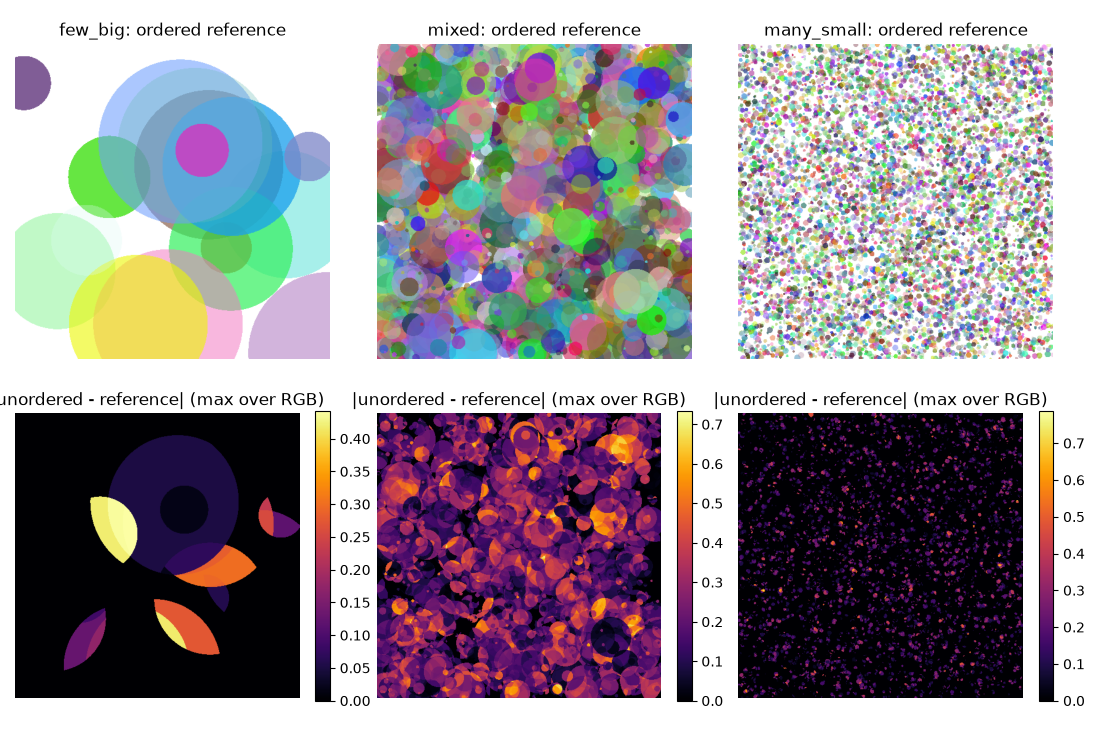
\includegraphics[width=0.92\linewidth]{render_order_error.png}
\caption{numpy 版：随机打乱圆的顺序（模拟按圆并行、不保序）与顺序参考之间的差。}\label{fig:cpu-order}
\end{figure}
\Cref{fig:cpu-order}：在 512 像素的 mixed 场景（2000 个圆）中，打乱顺序后 92\%--93\% 的像素误差超过 0.01。只有被至少两个圆覆盖、且这些圆的相对顺序被打乱的像素才会出错。
GPU naive kernel 的错误更严重（\cref{sec:naive}），因为它除了顺序错，还有读--改--写竞争。

\begin{figure}[H]\centering
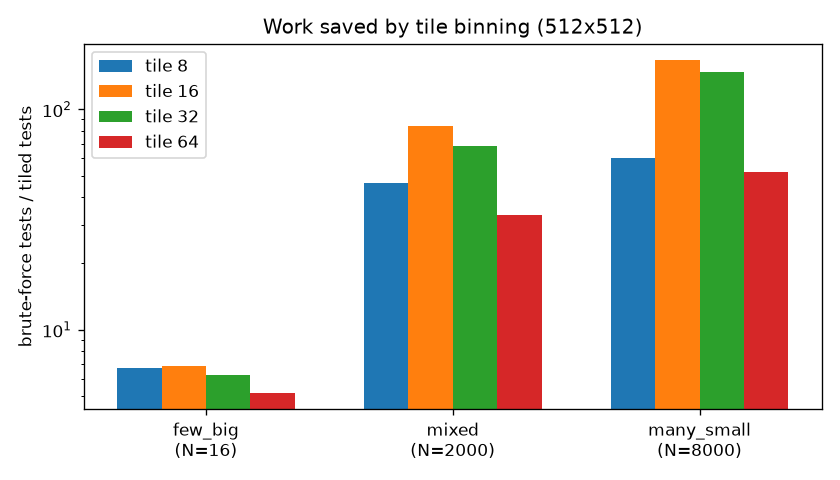
\includegraphics[width=0.7\linewidth]{render_binning_savings.png}
\caption{numpy 版：tile 分桶相对 brute force（每像素测试所有圆）省下的测试次数。}\label{fig:cpu-bin}
\end{figure}
\Cref{fig:cpu-bin}：many\_small（8000 个圆）在 tile=16 时测试次数比 brute force 少 167 倍。tile 太小时包围盒测试（圆数 $\times$ tile 数）占主导，
tile 太大时每个 tile 的圆列表变长。GPU 上的 tile 扫描（\cref{fig:tile}）结论相同，只是还要加上 launch、排序和 shared memory 容量的约束。

\subsection{Part 1：SAXPY——显存带宽与 PCIe}

\begin{figure}[H]\centering
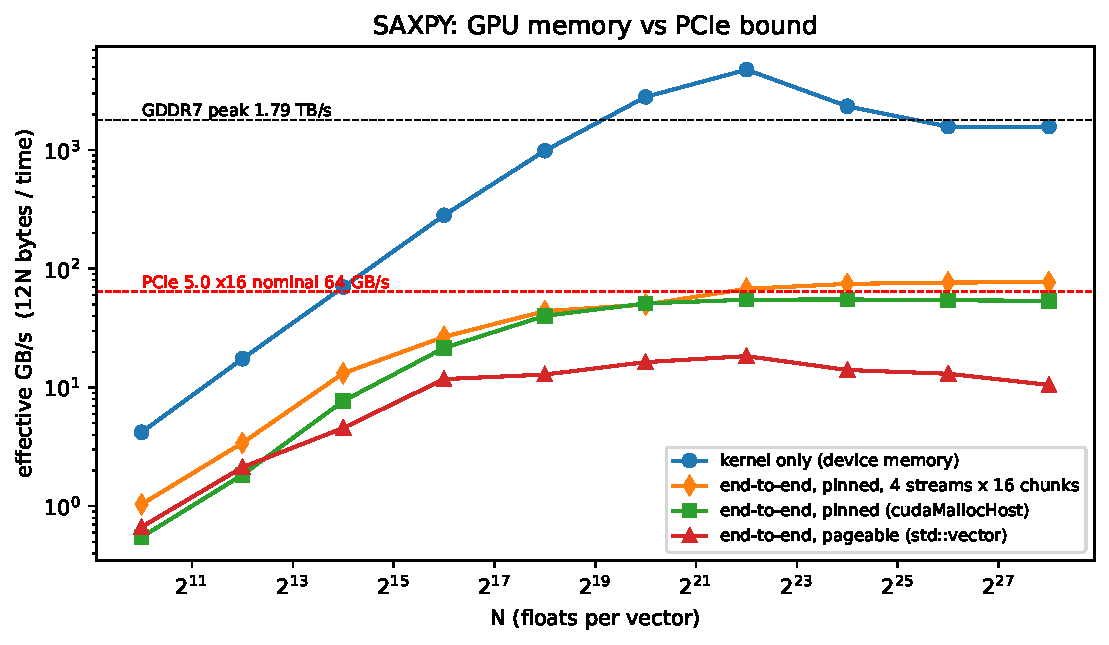
\includegraphics[width=0.85\linewidth]{gpu_saxpy_bandwidth.pdf}
\caption{SAXPY 有效带宽随 $N$ 的变化（\texttt{saxpy.jsonl}）。虚线分别为 GDDR7 标称带宽和 PCIe 5.0 x16 单向标称带宽。}\label{fig:saxpy}
\end{figure}

\Cref{fig:saxpy} 有四个区间：
\begin{itemize}
\item \textbf{$N\le 2^{14}$：launch 延迟主导。} kernel 时间几乎不变（$2^{10}$ 时 2.93\,$\mu$s，$2^{16}$ 时 2.78\,$\mu$s），所以带宽与 $N$ 成正比。
连续 launch 的间隔实测为 1.85\,$\mu$s，launch 加同步为 5.72\,$\mu$s。
\item \textbf{$2^{20}$--$2^{24}$：数据在 L2 内。} $N=2^{22}$ 时 kernel 达到 4759 GB/s，是 GDDR7 标称值的 2.7 倍。工作集 $12N=50$ MB，小于 96 MB 的 L2，
而且前面的 \texttt{cudaMemcpy} 已经把数据留在 L2 中。这是 L2 带宽，不是显存带宽。
\item \textbf{$N\ge 2^{26}$：显存带宽主导。} $2^{26}$ 和 $2^{28}$ 时 kernel 分别为 1577 和 1578 GB/s，是 1.79 TB/s 标称值的 88\%，与 asst1 测得的约 1.55 TB/s 一致。
\item \textbf{端到端由 PCIe 决定。} $2^{28}$ 时 pinned 端到端 53.8 GB/s，其中 H2D 56.5 GB/s、D2H 54.1 GB/s，约为 PCIe 5.0 x16 标称 64 GB/s 的 85\%–88\%。
pageable 只有 10.5 GB/s（H2D 10.8 GB/s）：驱动要先用 CPU 把数据拷到内部的 pinned staging 缓冲区，再做 DMA，瓶颈在主机端 memcpy。
streams 版达到 77.1 GB/s，\emph{超过}单向 PCIe 带宽，因为 PCIe 是全双工，H2D 和 D2H 可以同时进行。它的 41.8 ms 接近单独 H2D 的 38.0 ms，即时间下限为较长方向的拷贝时间。
\end{itemize}

\begin{figure}[H]\centering
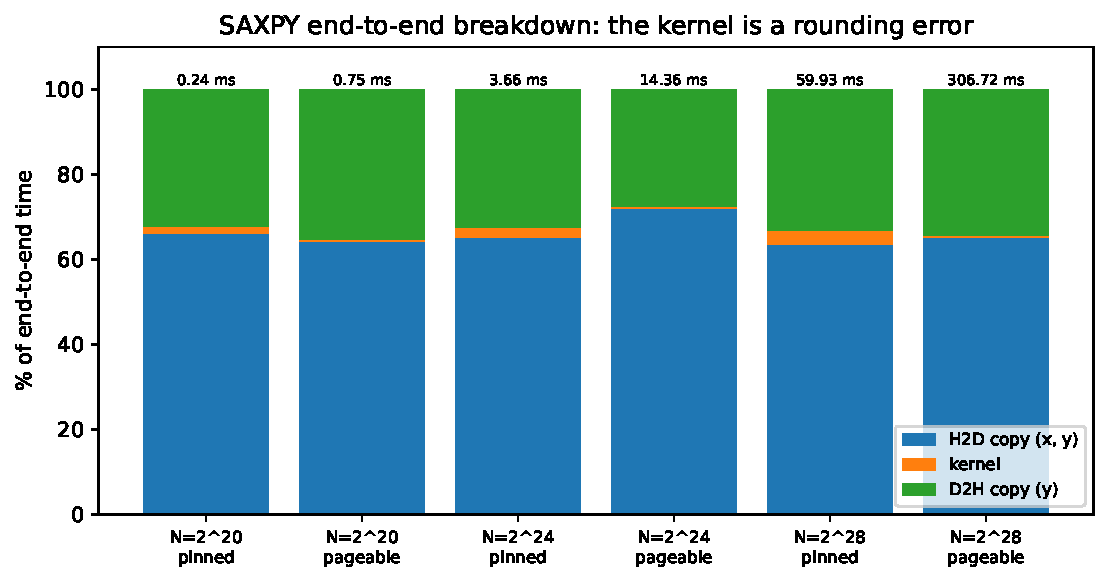
\includegraphics[width=0.8\linewidth]{gpu_saxpy_breakdown.pdf}
\caption{端到端时间分解（各段取中位数）。顶部数字为三段之和。}\label{fig:saxpy-break}
\end{figure}
\Cref{fig:saxpy-break}：$N=2^{28}$、pinned 时，H2D 38.04 ms、kernel 2.04 ms、D2H 19.85 ms，kernel 只占 3.4\%。H2D 搬 8N 字节、D2H 搬 4N 字节，所以 H2D 时间约为 D2H 的两倍。
pageable 下总时间为 306.7 ms，是 pinned 的 5.1 倍。

\begin{findingbox}[：SAXPY]
SAXPY 的算术强度是 $2/12\approx0.17$ FLOP/B，任何 GPU 上都受带宽限制。kernel 能用到 88\% 的 GDDR7 带宽，但只要数据需要从主机拷过来再拷回去，
瓶颈就变成 PCIe，比显存慢约 29 倍（1578 / 53.8）。对这类 kernel，GPU 加速的前提是数据常驻显存，或者在拷贝之后做足够多的计算来摊薄传输。
\end{findingbox}

\subsection{Part 2：exclusive scan}

\begin{figure}[H]\centering
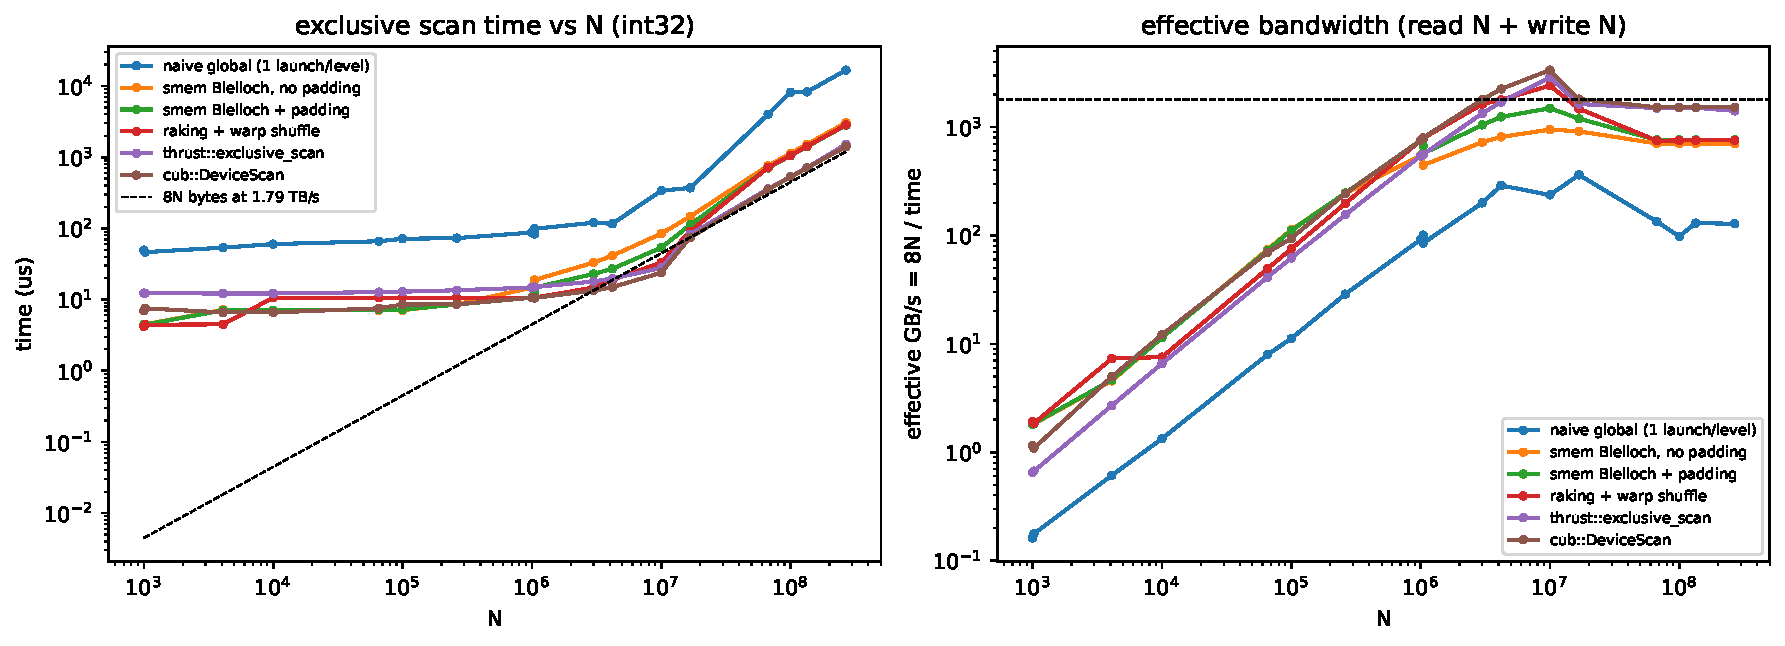
\includegraphics[width=\linewidth]{gpu_scan_time_bw.pdf}
\caption{六种 scan 的时间（左）和有效带宽 $8N/t$（右）。所有点 mismatch = 0。}\label{fig:scan}
\end{figure}

\Cref{fig:scan} 可以分成三段来读：
\begin{enumerate}
\item \textbf{大 $N$（$\ge 2^{26}$）。} $2^{28}$ 时 cub 1.412 ms（1521 GB/s）、thrust 1.522 ms、smem 2.817 ms（762 GB/s）、raking 2.839 ms、smem\_nopad 3.049 ms、naive 16.75 ms（128 GB/s）。
smem 和 raking 的有效带宽几乎正好是 cub 的一半。它们的第一遍读 $N$、写 $N$，\texttt{uniform\_add} 再读 $N$、写 $N$，实际流量是 $16N$ 字节；按 $16N$ 折算是 1.52 TB/s，与 cub 的 1.52 TB/s 相同。
也就是说，三者都已经跑在显存带宽上限，差别在于搬了多少字节。
\item \textbf{中等 $N$（$2^{22}$–$2^{24}$）。} 数据部分留在 L2 中，cub 在 $2^{24}$ 时有效带宽为 1816 GB/s，raking 为 1479 GB/s。
\item \textbf{小 $N$。} 时间不再随 $N$ 变化，见\cref{fig:latency}。
\end{enumerate}

\begin{figure}[H]\centering
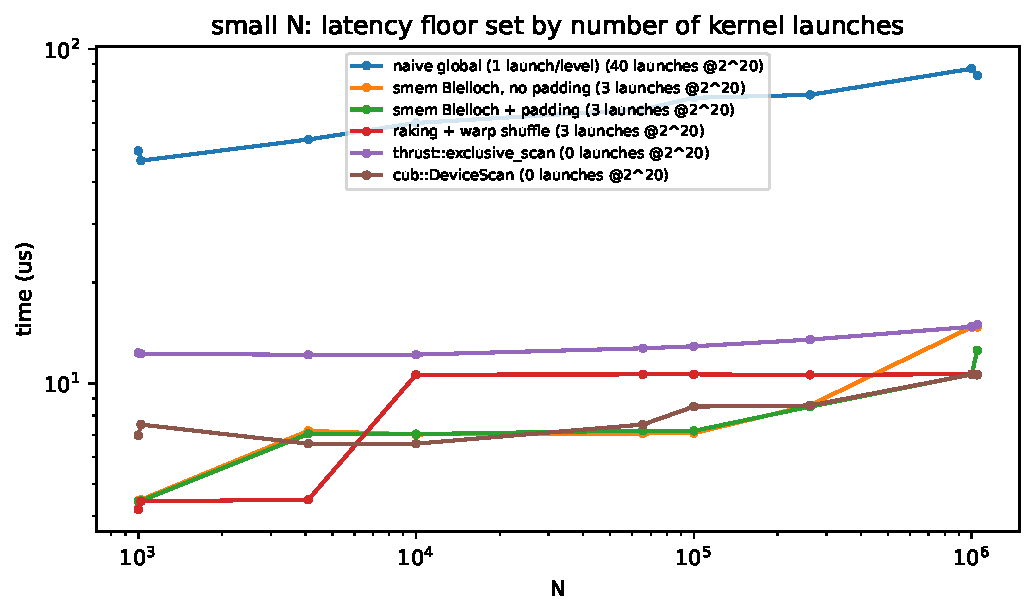
\includegraphics[width=0.75\linewidth]{gpu_scan_latency_floor.pdf}
\caption{$N\le2^{20}$ 时的延迟下限。图例中给出 $N=2^{20}$ 时各算法的 kernel launch 数（thrust/cub 内部的 launch 未计入）。}\label{fig:latency}
\end{figure}
\Cref{fig:latency}：$N=1000$ 时 naive 需要 20 次 launch 加一次 memcpy 和两次 memset，用时 49.55\,$\mu$s，平均每次操作约 2\,$\mu$s，与实测的 1.85\,$\mu$s 连续 launch 间隔一致。
单 block 的 smem 和 raking 只需一次 launch，用时 4.4\,$\mu$s；cub 需要两次 launch（初始化 tile 状态加 scan），用时 6.98\,$\mu$s；thrust 每次调用都要分配和释放临时缓冲，用时 12.3\,$\mu$s。
$N$ 从 1000 增加到 $2^{20}$（1000 倍），smem 版只从 4.43 变为 12.54\,$\mu$s，因为这段时间主要是固定开销。

\begin{figure}[H]\centering
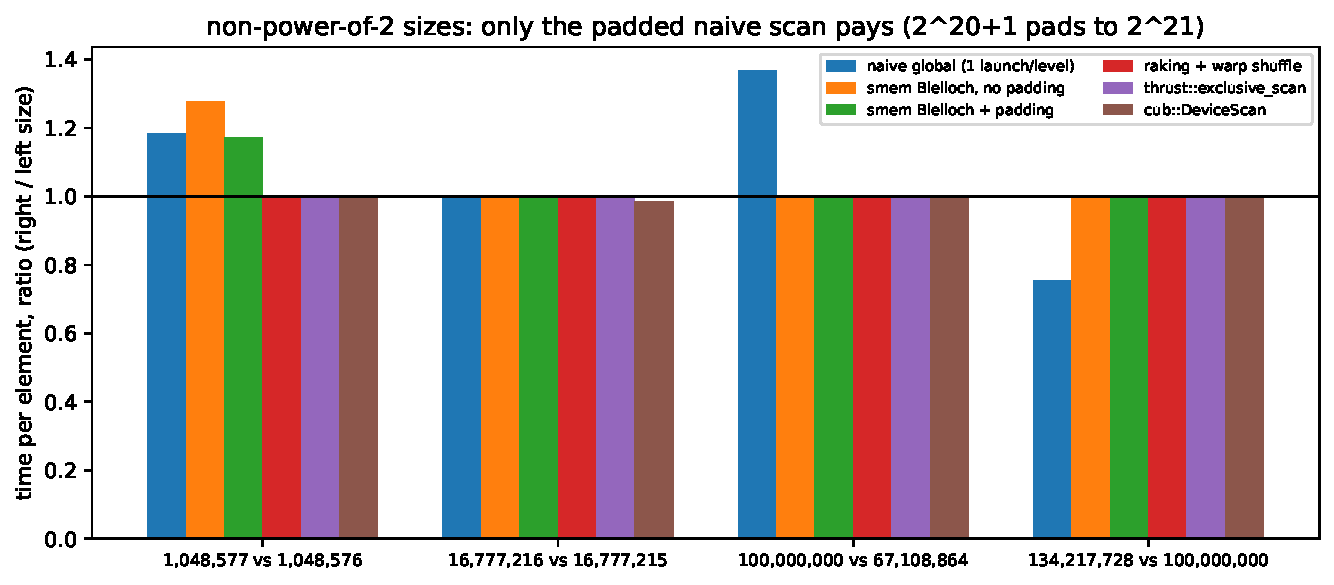
\includegraphics[width=0.9\linewidth]{gpu_scan_nonpow2.pdf}
\caption{非 2 的幂长度：每元素时间之比（右侧规模 / 左侧规模）。}\label{fig:nonpow2}
\end{figure}
\Cref{fig:nonpow2}：naive 必须补齐到 2 的幂。$10^8$ 补齐到 $2^{27}$，每元素时间是 $2^{26}$ 的 1.37 倍，与补齐比例 $2^{27}/10^8=1.34$ 相符；
$2^{27}$ 与 $10^8$ 的补齐长度相同，所以 $2^{27}$ 的每元素时间反而只有 $10^8$ 的 0.75 倍。分块算法不需要补齐，比值都约为 1.0。
唯一的例外是 $2^{20}+1$：smem 每块 1024 个元素，多出的 1 个元素会增加一个 block，块和数组的长度从 1024 变成 1025，因而多出一层递归（launch 数从 3 变为 5），在小规模下这多出的约 2\,$\mu$s 很明显。
raking 每块 4096 个元素，块和只有 257 个，不受影响。

\begin{table}[H]
\centering\small
\caption{scan kernel 的静态资源与理论 occupancy（\texttt{scan\_attrs.jsonl}；sm\_120 每 SM 最多 1536 线程）}\label{tab:scanattrs}
\begin{tabular}{lrrrrr}
\toprule
kernel & block & 寄存器 & 静态 smem (B) & blocks/SM & 理论 occupancy \\
\midrule
upsweep\_k & 256 & 10 & 0 & 6 & 1.00 \\
blelloch\_block（pad / nopad） & 512 & 18 & 4224 & 3 & 1.00 \\
raking\_block & 256 & 64 & 16928 & 4 & 0.67 \\
uniform\_add & 256 & 14 & 0 & 6 & 1.00 \\
\bottomrule
\end{tabular}
\end{table}
\Cref{tab:scanattrs}：raking 每线程在寄存器中保存 16 个元素，用到 64 个寄存器，占用率降到 0.67，但在 $2^{28}$ 时仍与 smem 一样快（2.839 和 2.817 ms），
说明这里的瓶颈不在 occupancy，而在 DRAM。padding 只多用 128 B shared memory（两种版本都按 4224 B 静态分配），却在 $2^{24}$ 时把时间从 146.9 降到 112.1\,$\mu$s（快 1.31 倍）。
因为 ncu 不可用，bank conflict 的次数没有直接计数，这个 1.31 倍是唯一的证据。

\begin{findingbox}[：scan]
在大规模下，scan 的快慢取决于读写显存的遍数，与 work 是 $2N$ 还是 $N$ 关系不大。naive 的问题是 launch 多和跨步访存，不是算法本身。
分块递归版本把流量降到 $16N$，单遍 decoupled look-back（cub）进一步降到 $8N$。在小规模下，决定时间的是 launch 次数，每次 launch 约 2\,$\mu$s。
\end{findingbox}

\begin{figure}[H]\centering
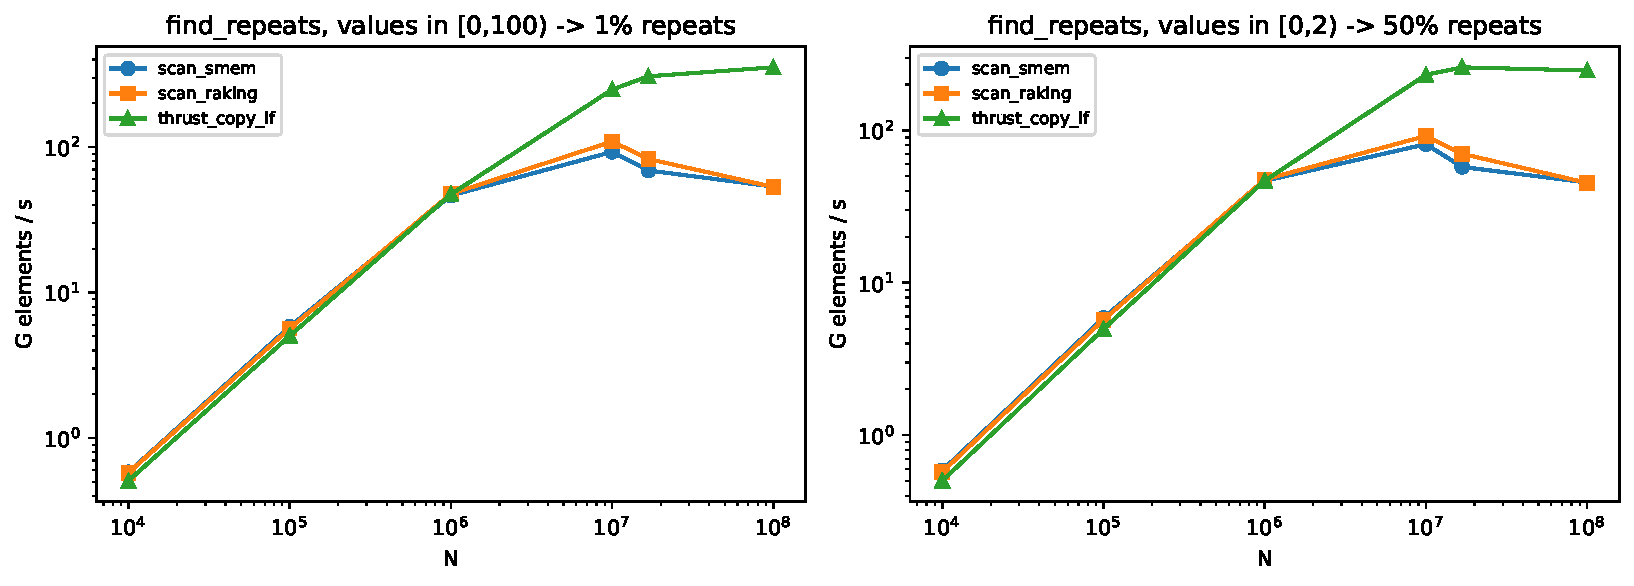
\includegraphics[width=\linewidth]{gpu_find_repeats.pdf}
\caption{\texttt{find\_repeats} 吞吐量（\texttt{find\_repeats.jsonl}），左：约 1\% 重复，右：约 50\% 重复。所有结果与 CPU 一致。}\label{fig:fr}
\end{figure}
\Cref{fig:fr}：$N\le10^6$ 时三者都在约 17--21\,$\mu$s，由 launch 和同步决定。自写版本要发 5 个以上 kernel 并做一次 4 字节 D2H，thrust 也要 D2H 取回输出个数。
$N=10^8$、1\% 重复时，自写 smem 版 1.869 ms，thrust 0.283 ms，后者快 6.6 倍。自写版本的流量估算为：flags 读 $a$ 写 $f$（$8N$）+ scan（$16N$）+ scatter 读 $a$ 和 $pos$（$8N$），共约 $32N=3.2$ GB，
按 1.87 ms 算是 1.71 TB/s，已经接近显存带宽上限~\cite{williams2009}。\texttt{copy\_if} 用单遍 look-back，把谓词计算和压缩合并在一个 kernel 中，基本只读一次 $a$（$4N$），流量少约 8 倍。
重复率为 50\% 时，thrust 从 0.283 ms 增加到 0.404 ms，因为要多写 $0.5N$ 个输出；自写版从 1.869 增加到 2.198 ms。

\begin{figure}[H]\centering
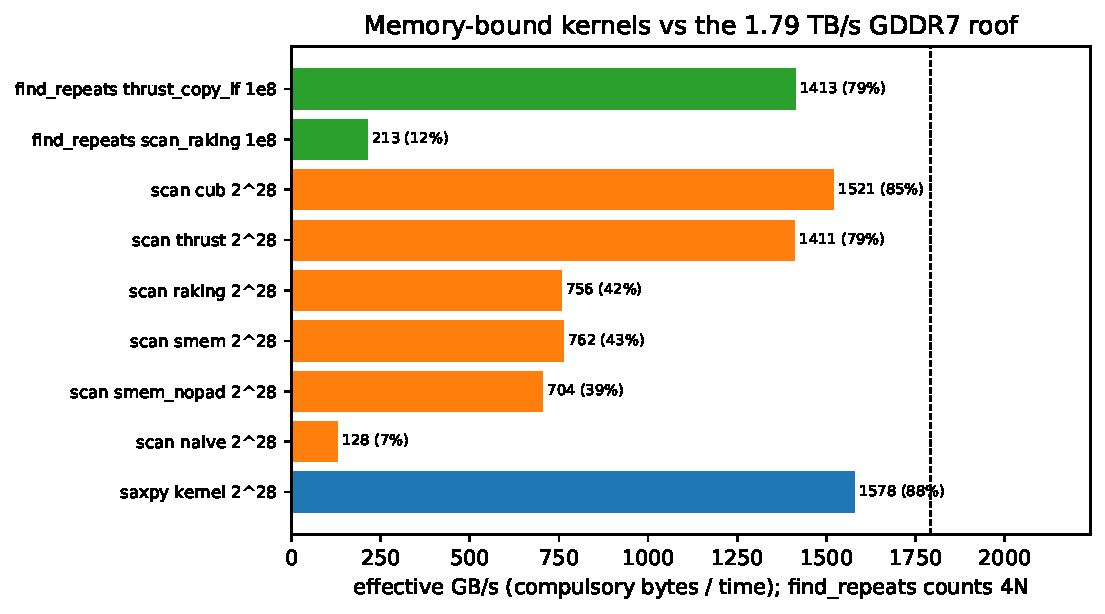
\includegraphics[width=0.8\linewidth]{gpu_bandwidth_roof.pdf}
\caption{访存受限 kernel 与 1.79 TB/s 上限对比（按算法必需的字节数计：scan 为 $8N$，find\_repeats 为 $4N$）。}\label{fig:roof}
\end{figure}
\Cref{fig:roof} 把各 kernel 放在同一根「必需字节数 / 时间」的轴上比较：SAXPY 88\%、cub 85\%、thrust scan 79\%、thrust copy\_if 79\%；自写 smem/raking 只有 42\%--43\%（nopad 39\%），因为实际流量是必需流量的两倍；naive 只有 7\%。
在这根轴上，离上限的距离就是多出来的访存遍数。

\subsection{Part 3：渲染器}

\begin{figure}[H]\centering
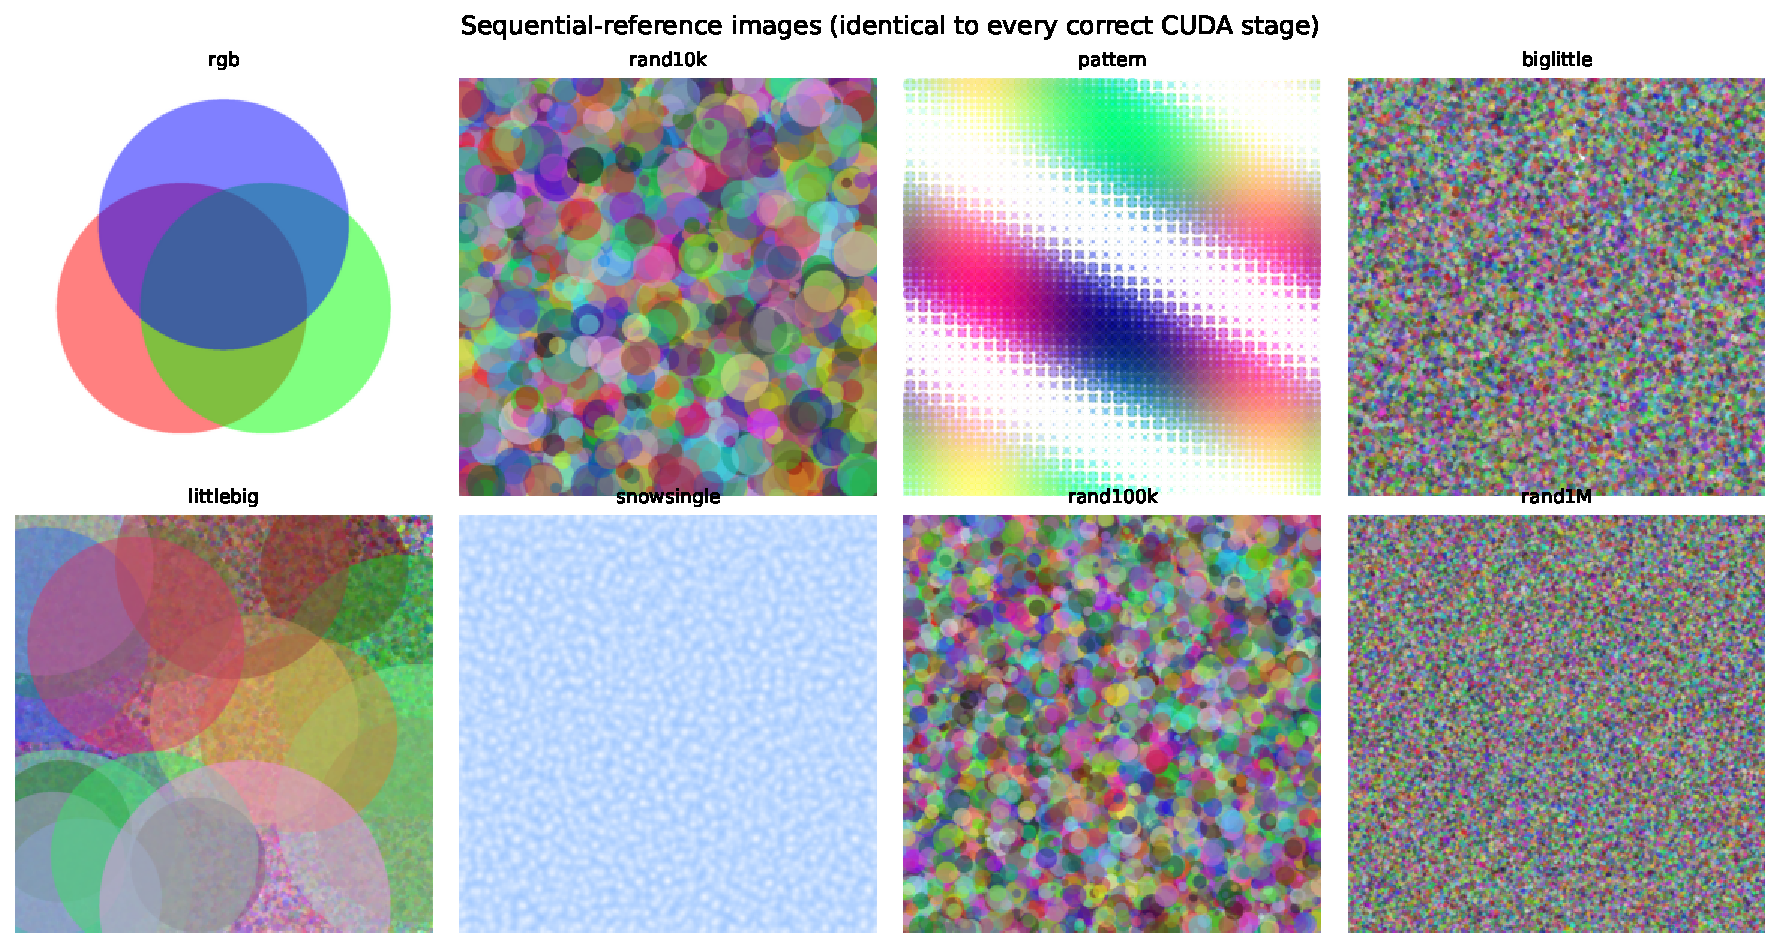
\includegraphics[width=\linewidth]{gpu_render_gallery.pdf}
\caption{CPU 顺序参考渲染结果（512 像素缩略图）。所有正确的 GPU 阶段与之逐位相同（snow 场景差 $\le2.98\times10^{-7}$）。}\label{fig:gallery}
\end{figure}

\subsubsection{(a) naive 一线程一圆是错的}\label{sec:naive}

\begin{figure}[H]\centering
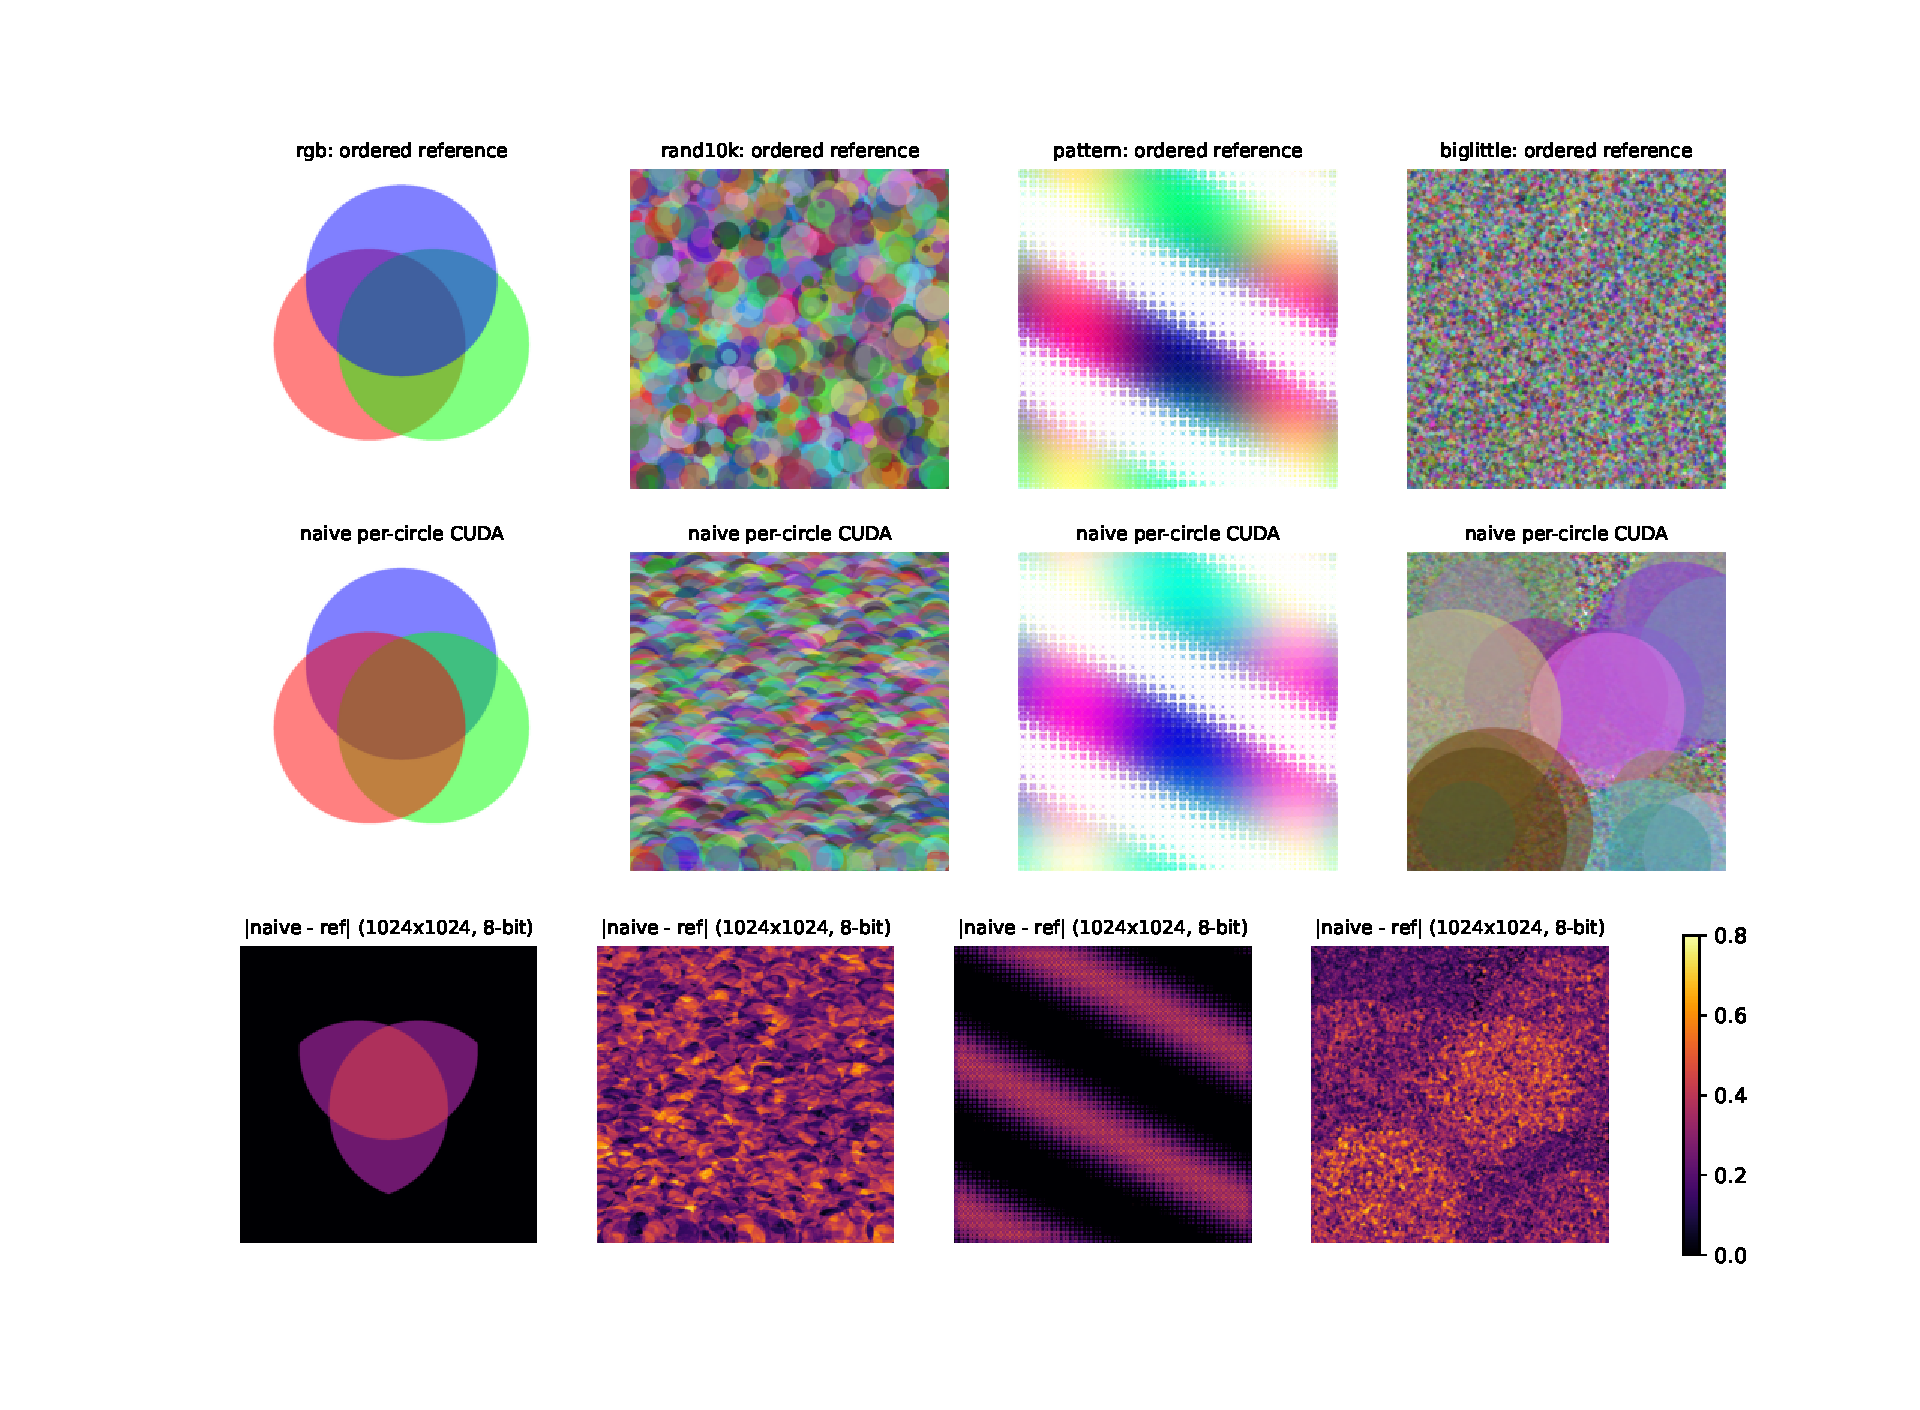
\includegraphics[width=0.95\linewidth]{gpu_render_naive_images.pdf}
\caption{上：顺序参考；中：naive CUDA；下：全分辨率逐像素最大通道差（8-bit 量化）。}\label{fig:naive-img}
\end{figure}

\begin{figure}[H]\centering
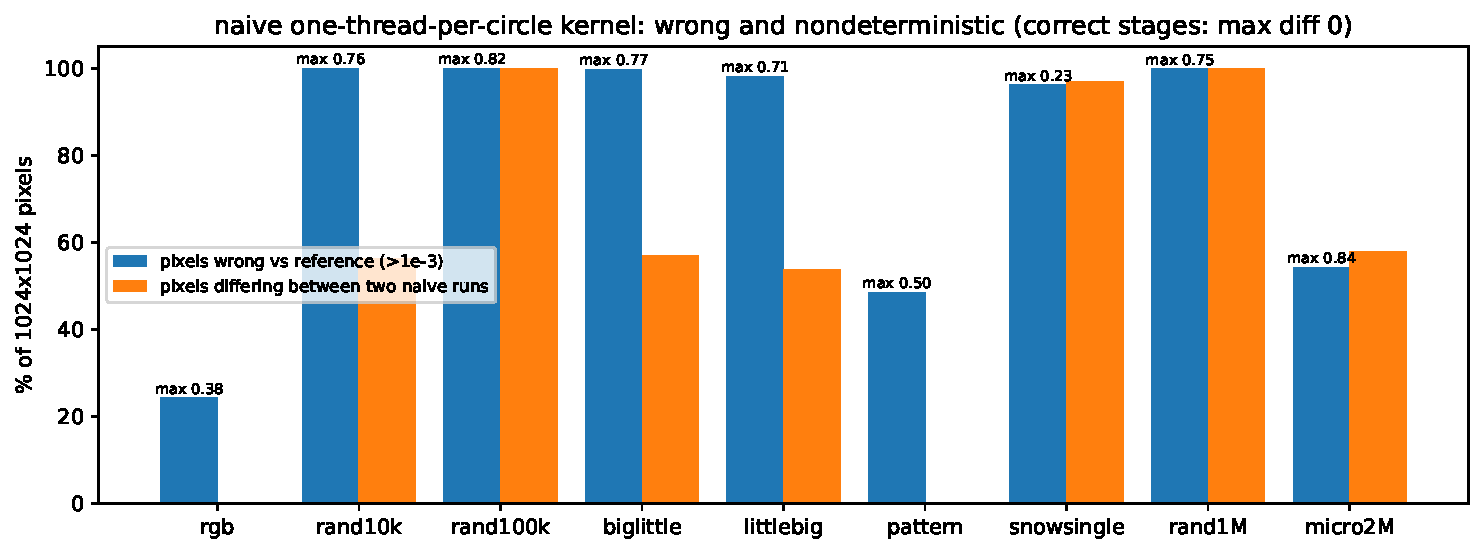
\includegraphics[width=0.9\linewidth]{gpu_render_naive_error.pdf}
\caption{naive kernel 的出错像素比例，以及两次运行结果不同的像素比例（\texttt{render.jsonl}）。}\label{fig:naive-err}
\end{figure}

\begin{table}[H]
\centering\small
\caption{naive 一线程一圆 kernel 的错误统计（共 1048576 个像素）}\label{tab:naive}
\begin{tabular}{lrrrr}
\toprule
场景 & 最大绝对误差 & 像素 $>10^{-6}$ & 像素 $>10^{-3}$ & 两次运行不同的像素 \\
\midrule
rgb & 0.375 & 254534 & 254534 & 0 \\
rand10k & 0.764 & 1048576 & 1048576 & 591059 \\
rand100k & 0.817 & 1048576 & 1048576 & 1048576 \\
biglittle & 0.767 & 1045372 & 1045372 & 597239 \\
littlebig & 0.710 & 1029479 & 1029381 & 564817 \\
pattern & 0.505 & 508748 & 508334 & 1462 \\
snowsingle & 0.232 & 1048515 & 1008719 & 1017242 \\
rand1M & 0.754 & 1048385 & 1047349 & 1048518 \\
micro2M & 0.840 & 589547 & 569401 & 608102 \\
\bottomrule
\end{tabular}
\end{table}

\Cref{fig:naive-img,fig:naive-err,tab:naive} 显示了两种不同的错误：
\begin{itemize}
\item \textbf{只有顺序错误，结果是确定的。} rgb 场景的三个圆在同一个 warp 中，三条 lane 以 lockstep 方式各自遍历自己的包围盒。同一像素在不同循环迭代中被访问，先后由包围盒的几何形状决定，与输入顺序无关。
因此 24.3\% 的像素出错，但两次运行结果完全一样（0 个像素不同）。这个例子说明，结果可复现并不代表正确。
\item \textbf{读--改--写竞争。} 其余场景中，不同 warp、不同 SM 同时读写同一像素，有的更新被覆盖丢失，有的顺序随机。rand100k 两次运行的所有像素都不同。
biglittle 的 naive 图中大圆浮在最上层（\cref{fig:naive-img} 第 4 列）：大圆对应的线程循环最长，最后才写完，所以它们的写入覆盖了小圆。这与输入顺序（大圆在底层）正好相反。
\item pattern 场景重叠少（平均覆盖 1.9），只在圆有重叠的斜带上出错，48.5\% 的像素错，两次运行只有 1462 个像素不同：大部分错误来自确定的顺序，少量来自竞争。
\end{itemize}

\subsubsection{(b) 正确且快：各优化阶段}

\begin{table}[H]
\centering\small
\caption{每帧时间（ms，取各阶段在不同 tile 下的最优值，括号内为 tile 大小）。加速比为 CPU 参考除以最快的正确 GPU 阶段。}\label{tab:render}
\setlength{\tabcolsep}{2.6pt}
\begin{tabular}{lrrrrrrrrr}
\toprule
场景 & $N$ & 覆盖 & CPU & naive（错误率） & allcircles & binned & binned\_smem & blockscan & 加速比 \\
\midrule
rgb & 3 & 0.8 & 7.4 & 46.518 (24.3\%) & 0.015 & 0.049 (32) & 0.047 (32) & 0.015 (16) & 506 \\
rand10k & 10000 & 44.9 & 129.9 & 2.837 (100.0\%) & 8.322 & 0.165 (16) & 0.136 (16) & 0.150 (32) & 952 \\
rand100k & 100000 & 112.6 & 422.7 & 2.782 (100.0\%) & 84.532 & 0.411 (16) & 0.303 (16) & 1.008 (32) & 1393 \\
biglittle & 50020 & 10.4 & 45.4 & 58.206 (99.7\%) & 41.930 & 0.141 (16) & 0.121 (16) & 0.404 (32) & 375 \\
littlebig & 50020 & 10.7 & 45.4 & 52.800 (98.2\%) & 41.927 & 0.140 (16) & 0.120 (16) & 0.406 (32) & 378 \\
pattern & 5120 & 1.9 & 6.0 & 0.838 (48.5\%) & 4.263 & 0.074 (16) & 0.070 (16) & 0.047 (32) & 126 \\
snowsingle & 50000 & 39.2 & 393.3 & 1.841 (96.2\%) & 22.472 & 0.258 (16) & 0.201 (16) & 0.533 (32) & 1957 \\
rand1M & 1000000 & 59.7 & 383.3 & 2.109 (99.9\%) & 844.282 & 0.587 (8) & 0.538 (16) & 7.591 (32) & 712 \\
micro2M & 2000000 & 6.8 & 147.8 & 0.638 (54.3\%) & 1690.730 & 0.463 (8) & 0.505 (8) & 14.239 (32) & 319 \\
\bottomrule
\end{tabular}
\end{table}

\begin{figure}[H]\centering
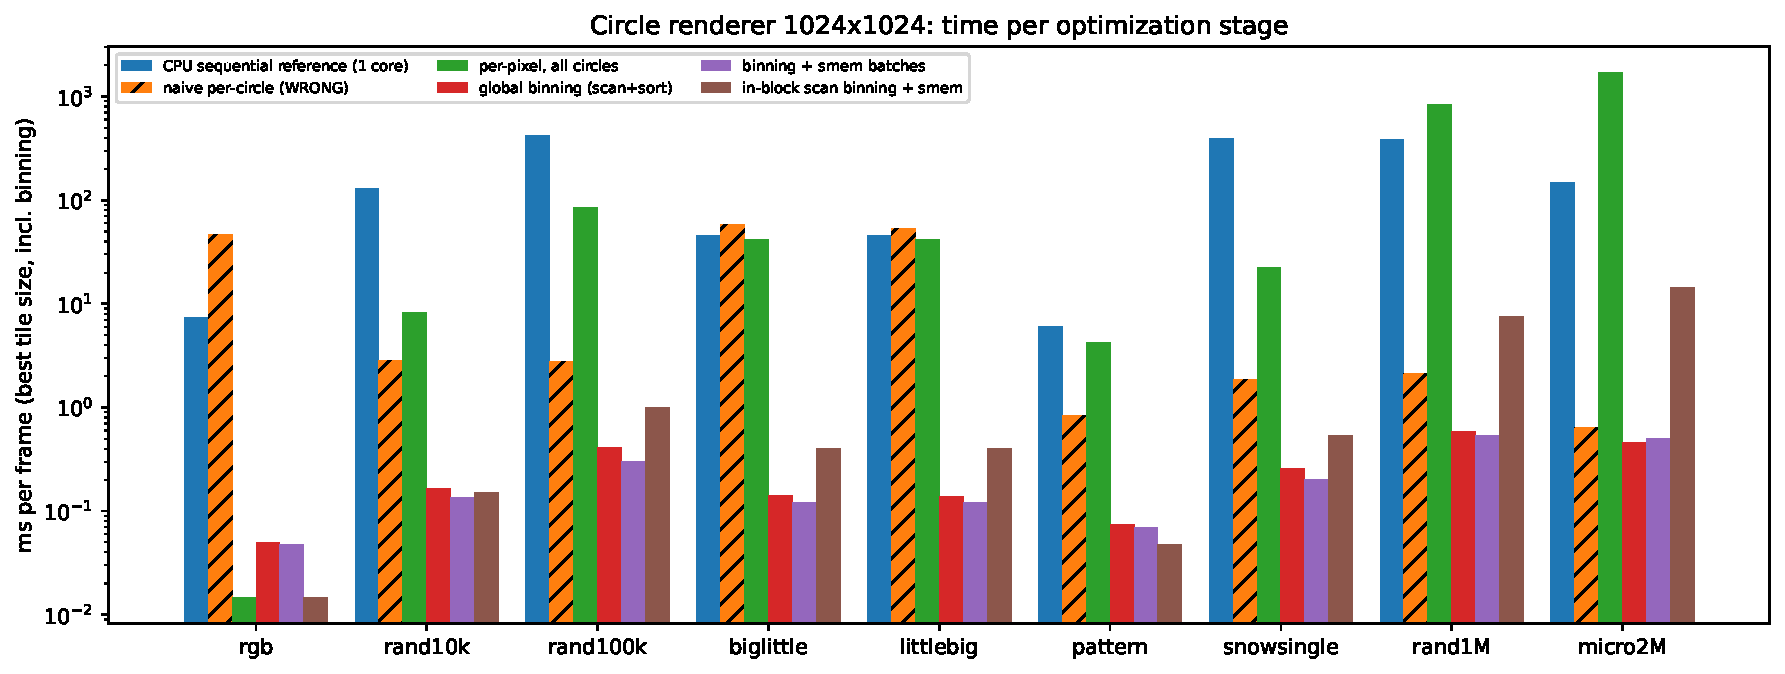
\includegraphics[width=\linewidth]{gpu_render_stages.pdf}
\caption{各优化阶段的每帧时间（对数轴，最优 tile，包含分桶时间）。}\label{fig:stages}
\end{figure}

\Cref{tab:render,fig:stages} 的读法：
\begin{itemize}
\item \textbf{allcircles 正确，但工作量是 $O(NP)$。} rand1M 有 $1.05\times10^{12}$ 次圆--像素测试，用时 844 ms，约为每秒 $1.24\times10^{12}$ 次测试，比单核 CPU 参考（383 ms）还慢。
CPU 参考只测包围盒内的像素，工作量与覆盖面积成正比，而不是与 $NP$ 成正比。
\item \textbf{binned 把测试数降到 $P\times\overline{L}$}，$\overline{L}$ 为每个 tile 的平均列表长度。rand1M 在 $T=16$ 时 $\overline{L}=609.5$，只需 $6.39\times10^8$ 次测试，是 allcircles 的 1/1640。
render kernel 0.385 ms，约为每秒 $1.66\times10^{12}$ 次测试。单次测试的吞吐与 allcircles 差不多，加速几乎全部来自测试次数的减少。
\item \textbf{shared memory 批量取圆}（binned $\to$ binned\_smem）。在 $T\ge16$ 时有效：rand100k $T=32$ 的 render 时间从 0.502 降到 0.293 ms（1.71 倍），rand1M $T=32$ 从 1.772 降到 0.849 ms（2.09 倍）。
有两个原因：每个圆的 7 个参数每个 block 只从 global memory 读一次；寄存器从 52 个降到 34 个（\cref{tab:renderattrs}），256 线程块的理论 occupancy 从 0.67 升到 1.0。
$T=8$ 时每批只有 64 个圆，加上同步开销，没有收益。
\item \textbf{blockscan} 只有一次 launch，没有全局排序，在 $N$ 小的场景最快（rgb 0.015 ms，pattern 0.047 ms）。但它的工作量是 tile 数 $\times N$ 次包围盒测试，
micro2M 在 $T=16$ 时是 $4096\times2\times10^6=8.2\times10^9$ 次，用时 28.8 ms，比 binned 慢 30 倍以上。
\end{itemize}

\begin{figure}[H]\centering
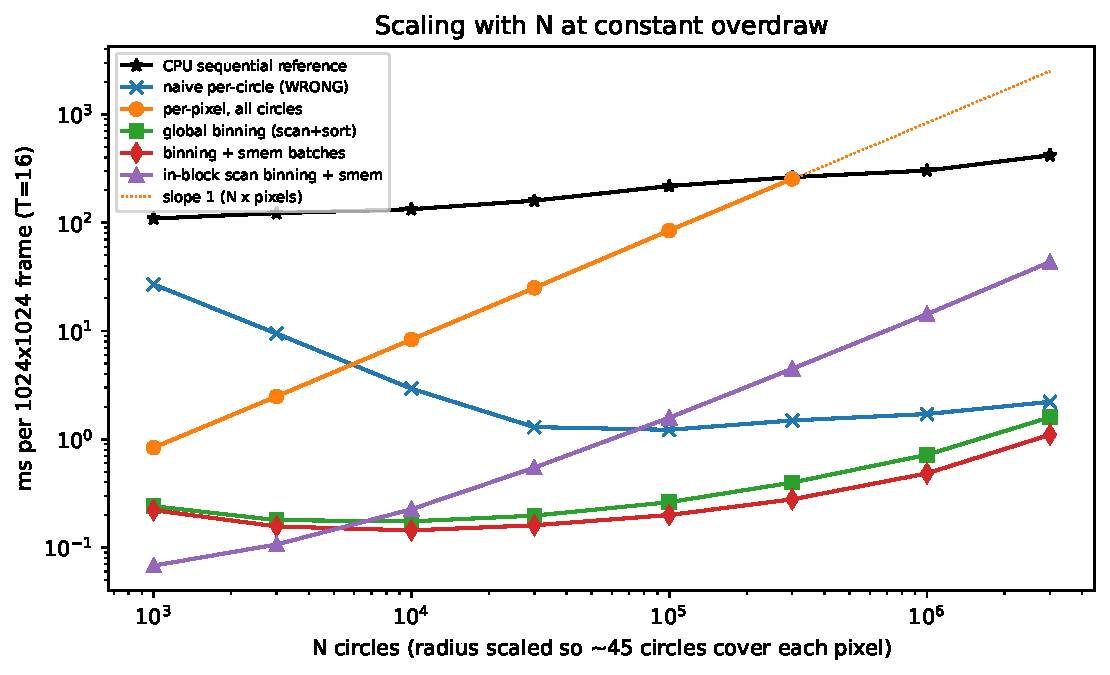
\includegraphics[width=0.8\linewidth]{gpu_render_sweep.pdf}
\caption{overdraw 固定为约 45、$N$ 从 $10^3$ 到 $3\times10^6$（\texttt{render\_sweep.jsonl}，$T=16$）。allcircles 在 $N>3\times10^5$ 时不再运行。}\label{fig:sweep}
\end{figure}
\Cref{fig:sweep} 把渐近行为分开来看：allcircles 的斜率为 1（$N$ 每增加 10 倍，时间也增加约 10 倍：$10^4$ 时 8.33 ms，$10^5$ 时 84.6 ms），在 $3\times10^5$ 时与 CPU 相当（253.8 和 263.3 ms）。
blockscan 的斜率也接近 1，因为它测试的是 tile 数 $\times N$。binned\_smem 在 $N$ 增加 3000 倍的过程中只从 0.222 ms 增加到 1.101 ms：总覆盖面积不变，渲染工作量基本不变，增加的是分桶开销和随 $N$ 变长的列表（圆变小后，跨 tile 的包围盒占比上升）。
两条曲线的交点在 $N\approx5000$：$N=3000$ 时 blockscan 更快（0.107 和 0.157 ms），$N=10^4$ 时 binned\_smem 更快（0.144 和 0.226 ms）。
CPU 参考的时间与 $N$ 关系不大（109--418 ms），因为它的工作量同样与覆盖面积成正比。

\subsubsection{分桶开销、列表长度与 tile 大小}

\begin{figure}[H]\centering
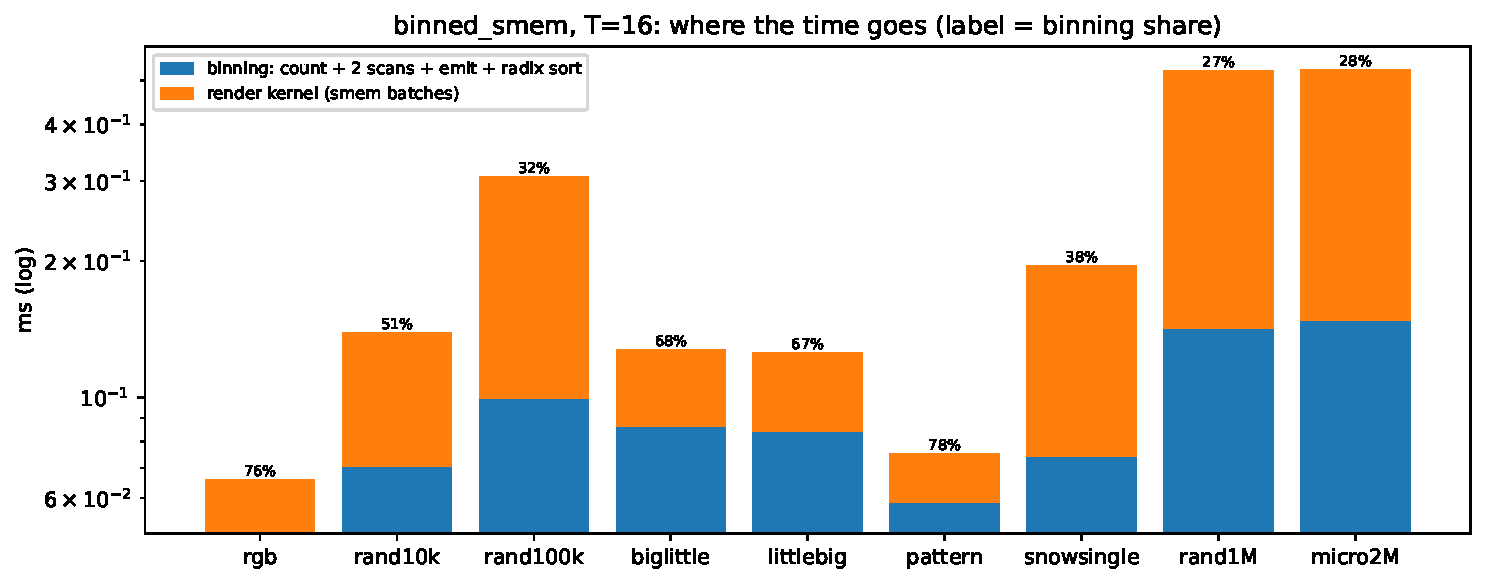
\includegraphics[width=0.85\linewidth]{gpu_render_breakdown.pdf}
\caption{binned\_smem 在 $T=16$ 时分桶与渲染的时间分解。}\label{fig:break}
\end{figure}
\Cref{fig:break}：分桶时间大致在 0.05--0.15 ms，下限是 6 次 launch、2 次 D2H 同步加一次 radix sort。rgb 只有 3 个圆，分桶仍需 0.050 ms，占总时间的 82\%；
而且每个大圆要由单个线程把覆盖的约 1500 个 tile 依次 \texttt{atomicAdd} 和 emit，这是一线程一圆分桶在大圆上的负载不均衡。
在 rand1M 和 micro2M 中，渲染占 72\% 和 65\%（0.385 和 0.380 ms），分桶的固定成本被摊薄。

\begin{figure}[H]\centering
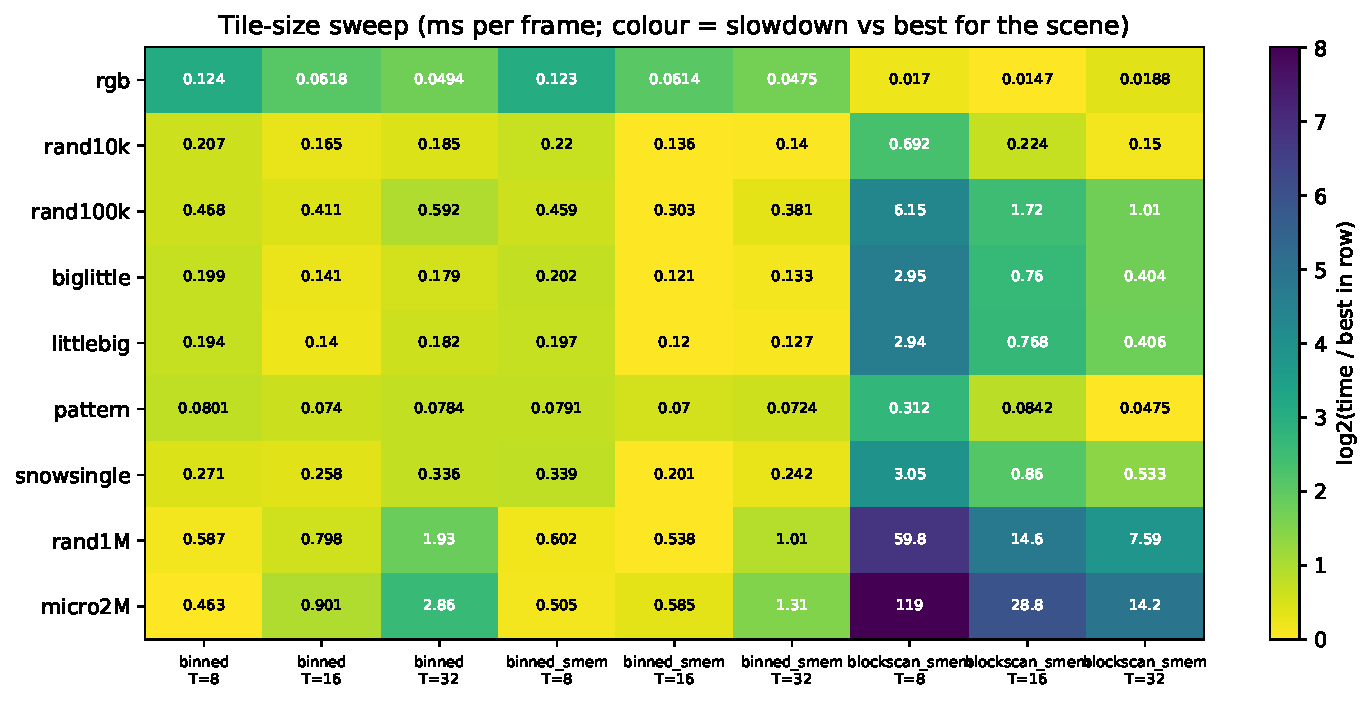
\includegraphics[width=\linewidth]{gpu_render_tile_sweep.pdf}
\caption{tile 大小扫描。格内为每帧 ms，颜色为相对该场景最优值的 $\log_2$ 慢速比。}\label{fig:tile}
\end{figure}
\begin{figure}[H]\centering
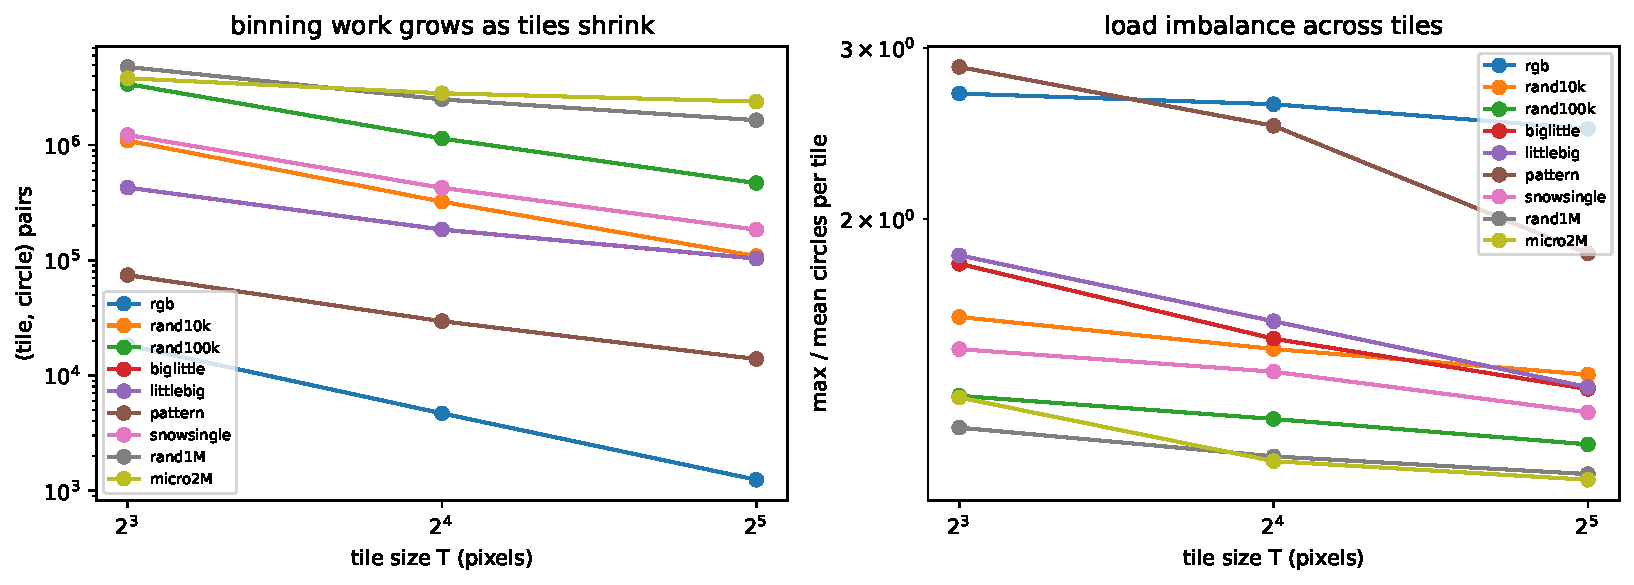
\includegraphics[width=\linewidth]{gpu_render_lists.pdf}
\caption{左：(tile, circle) 对的数量；右：最长列表与平均列表长度之比（负载不均衡程度）。}\label{fig:lists}
\end{figure}
\Cref{fig:tile,fig:lists}：tile 越小，(tile, circle) 对越多（rand10k 在 $T=8$ 时 1093947 对，$T=32$ 时 108651 对），分桶工作量越大；tile 越大，每个像素要遍历的列表越长。
micro2M 的圆半径约 1 像素，列表长度近似与 tile 面积成正比：$T=8,16,32$ 时分别为 232、689、2332，所以 $T=8$ 最快（binned 0.463 ms），$T=32$ 慢 6.2 倍（2.858 ms）。
只有 3 个大圆的 rgb 在 $T=32$ 时最快（binned\_smem 0.047 ms），因为每个圆本来就跨很多 tile，小 tile 只会增加对的数量。
对 blockscan 来说，tile 越大，tile 数越少，包围盒测试的总量就越少（tile 数 $\times N$），所以除 rgb（$N=3$，测试量可以忽略）外，都是 $T=32$ 最快。
负载均衡方面，max/mean 在 rand 类场景中为 1.1--1.6 倍，均衡情况良好；rgb 和 pattern 有大面积空白 tile 与重叠区并存，为 1.8--2.9 倍。

\begin{table}[H]
\centering\small
\caption{渲染 kernel 的资源占用（\texttt{render\_attrs.jsonl}；smem 版的动态 shared memory 为 $7\times$ blockDim $\times$ 4 B）}\label{tab:renderattrs}
\setlength{\tabcolsep}{4pt}
\begin{tabular}{lrrrrr}
\toprule
kernel & 寄存器 & 256 线程：blocks/SM & occupancy & 1024 线程：smem (B) & occupancy \\
\midrule
k\_naive & 52 & 4 & 0.67 & 0 & 0.67 \\
k\_allcircles & 40 & 6 & 1.00 & 0 & 0.67 \\
k\_bin\_count / k\_bin\_emit & 22 / 40 & 6 & 1.00 & 0 & 0.67 \\
k\_render\_binned & 52 & 4 & 0.67 & 0 & 0.67 \\
k\_render\_binned\_smem & 34 & 6 & 1.00 & 28672 & 0.67 \\
k\_render\_blockscan & 34 & 6 & 1.00 & 28672 & 0.67 \\
\bottomrule
\end{tabular}
\end{table}
\Cref{tab:renderattrs}：1024 线程块（$T=32$）每个 SM 只能放一个，occupancy 上限为 1024/1536=0.67，所以 $T=32$ 本身就比 $T=16$ 的 6 个 256 线程块（1.0）吃亏。

\begin{findingbox}[：渲染器]
保序的关键是把并行轴从「圆」换成「像素 / tile」，并用 scan 计算偏移、生成每个 tile 内仍按输入顺序排列的圆列表。之后每个像素在寄存器中按顺序混合，既不需要原子操作，也不需要锁。
从 allcircles 到 binned 的加速来自测试次数减少（rand1M 少 1640 倍）；shared memory 批量取圆再带来 1.3--2.1 倍；tile 大小要根据圆半径选：小圆选小 tile，大圆选大 tile。
在本测试集中 $T=16$ 是最稳妥的默认值，9 个场景里有 7 个的 binned\_smem 最优值落在 $T=16$。
\end{findingbox}

%=====================================================================
\section{与理论模型的对照}

\subsection{SAXPY：屋顶线与 PCIe}
算术强度 $I=2/12=0.167$ FLOP/B。RTX 5090 的 FP32 峰值约 105 TFLOP/s（厂商规格），屋脊点约为 $105\times10^{12}/1.79\times10^{12}\approx58$ FLOP/B，SAXPY 远在其左侧。kernel 时间的预测为
\[
t_\text{kernel}=\frac{12N}{B_\text{DRAM}}=\frac{3.22\ \text{GB}}{1.79\ \text{TB/s}}=1.80\ \text{ms}\quad(\text{实测 }2.04\ \text{ms，88\%}).
\]
端到端时间的预测（使用实测的单向带宽）：
\[
t_\text{e2e}=\frac{8N}{B_\text{H2D}}+t_\text{kernel}+\frac{4N}{B_\text{D2H}}
=\frac{2.147}{56.45}+2.04+\frac{1.074}{54.10}\ \text{ms}=38.0+2.0+19.8=59.9\ \text{ms},
\]
与实测的 59.91 ms 一致（这几个量都取自同一行数据，所以是自洽性检查）。拷贝和计算完全流水化时，时间下限为 $\max(8N/B_\text{H2D},4N/B_\text{D2H})=38.0$ ms，实测 streams 为 41.8 ms，差距是首尾块无法重叠的部分。

\subsection{scan：访存遍数模型}
设持续显存带宽为 $B=1.52$ TB/s（取 cub 在 $2^{28}$ 时的值）。
\begin{align*}
\text{cub（单遍 look-back）}: &\ 8N\ \text{B} \Rightarrow 2.147\ \text{GB}/B = 1.41\ \text{ms}\quad(\text{实测 }1.412)\\
\text{smem / raking（两遍 + 递归）}: &\ 16N\ \text{B} \Rightarrow 2.82\ \text{ms}\quad(\text{实测 }2.817\ /\ 2.839)\\
\text{naive（逐层跨步）}: &\ \approx 84N\ \text{B} \Rightarrow 14.8\ \text{ms}\quad(\text{实测 }16.75)
\end{align*}
naive 的 $84N$ 是这样估算的。DRAM 和 L2 的访问粒度是 32 B 的 sector（8 个 int）。stride $s=2^{d+1}<16$ 的前三层几乎连续访问，每层约读写整个数组（$8N$ 字节），up-sweep 和 down-sweep 合计约 $48N$。
$s\ge16$ 的层中，每个线程的两个地址落在不同 sector：up-sweep 读 2 个、写 1 个 sector（96 B），down-sweep 读 2 个、写 2 个（128 B）。线程数为 $N/s$，求和 $\sum_{s\ge16}1/s=1/8$，
这部分合计 $(96+128)N/8=28N$。再加上初始复制 $8N$，总计约 $84N$。实测比估算慢 13\%，多出的部分包括 56 次 launch（约 0.1 ms）和深层访问的 DRAM 行局部性较差。
这个模型说明，naive 慢的主要原因是跨步访问浪费 sector，从 work（加法次数）上看不出这一点。

\paragraph{work 与 span 在 GPU 上对应什么。} numpy 版统计的 span $=2\log_2 m$，在 naive GPU 版中就是 $2\log_2 m$ 次 launch。按每次约 2\,$\mu$s 计，
$N=2^{20}$ 时的下限约为 $40\times2=80\,\mu$s，实测 83.3\,$\mu$s，可见 naive 在 $2^{20}$ 时完全由 span（launch 次数）决定。
分块版本把 span 的大部分放到块内用 \texttt{\_\_syncthreads} 完成（代价是几十纳秒而不是微秒），跨块的同步只剩递归层数（$\log_{1024}N$），launch 数为 3--5 次。
Brent~\cite{brent1974} 定理 $T_P\le W/P+S$ 依然成立，只是在 GPU 上，跨块的 $S$ 每一步要乘以约 2\,$\mu$s，而块内的每一步只是一次 barrier。

\subsection{渲染器的成本模型}
设 $P$ 为像素数，$N$ 为圆数，$T$ 为 tile 边长，$\overline{L}(T)$ 为平均每 tile 的列表长度，$c$ 为平均覆盖数：
\begin{align*}
t_\text{allcircles} &\approx \frac{P\,N}{R_\text{test}}, &
t_\text{binned} &\approx t_\text{bin}(N,\#\text{pairs}) + \frac{P\,\overline{L}(T)}{R_\text{test}}, &
t_\text{blockscan} &\approx \frac{(P/T^2)\,N}{R_\text{bbox}} + \frac{P\,\overline{L}(T)}{R_\text{test}},
\end{align*}
对于半径为 $r$ 像素的圆，$\overline{L}(T)\approx c\,(1+2r/T)^2$。由 rand1M 数据可得 $R_\text{test}\approx1.2$--$1.7\times10^{12}$/s；
由 micro2M 的 blockscan（$T=16$，$8.2\times10^9$ 次包围盒测试，28.8 ms）可得 $R_\text{bbox}\approx2.8\times10^{11}$/s。按这个模型，
blockscan 与 binned 的交点在 $N\,P/T^2\approx R_\text{bbox}\cdot t_\text{bin}$，即 $N\approx2.8\times10^{11}\times10^{-4}\ \text{s}/4096\approx7000$（$T=16$、$t_\text{bin}\approx0.1$ ms），
与 sweep 实测的约 5000 处于同一量级。

%=====================================================================
\section{面试专题}

\paragraph{20 秒讲法。} 「我在 RTX 5090 上复刻了 CS149 作业 3。SAXPY 的 kernel 能跑到显存带宽的 88\%，但加上 PCIe 拷贝后只剩 54 GB/s，kernel 只占 3\% 的时间。
scan 上，我写的分块版本和 cub 都已经跑在显存带宽上限，cub 快一倍，是因为它只读写一遍。渲染器的难点是保序：一线程一圆的写法在 9 个场景里有 24\% 到 100\% 的像素出错。
我改成按 tile 并行，用 scan 和稳定排序为每个 tile 生成按输入顺序排列的圆列表，再用 shared memory 分批取圆。结果与 CPU 参考逐位相同，rand1M 比 CPU 快 712 倍。」

\paragraph{STAR 故事。}
\textbf{S}：渲染器有两个正确性约束（原子、保序）；starter 的一线程一圆 kernel 在 rand10k 上全部 1048576 个像素出错，两次运行有 591059 个像素不同。
\textbf{T}：在逐位正确的前提下，让 rand1M、micro2M 这类上百万个圆的场景达到亚毫秒级。
\textbf{A}：先写一线程一像素、遍历全部圆的版本，确认可以做到逐位正确（为此加了 \texttt{-fmad=false}，并让 host 和 device 共用 \texttt{shade()}）；再加上基于 scan 的全局分桶和稳定 radix sort；
接着用 shared memory 分批取圆，把寄存器数从 52 降到 34；最后扫描 tile 大小，并加了一个 overdraw 固定、$N$ 变化的 sweep 来区分各方法的渐近行为。
\textbf{R}：rand1M 从 844 ms 降到 0.538 ms（1569 倍），比 CPU 参考快 712 倍；90 个 (场景, 阶段, tile) 组合全部通过逐像素比较；
同时发现 blockscan 在 $N\lesssim5000$ 时更快，tile 大小应按圆半径选择。

\begin{iqbox}{为什么一线程一圆、每像素加 atomic 也不对？}
\textbf{答}：atomic 只保证一次「读--改--写」不被打断，不保证不同圆之间的先后顺序。over 混合（\cref{eq:over}）不满足交换律，两个 $\alpha=0.5$ 的圆交换顺序后，像素颜色就不同。
另外 float4 颜色没有现成的原子 over 操作，需要用 CAS 循环或锁来实现，而且仍然无法保序。正确的做法是按像素并行，每个像素按顺序遍历覆盖它的圆。
\par\textbf{常见错答}：「加 \texttt{atomicAdd} 就好了。」加法满足交换律，over 不满足；rgb 场景即使没有竞争（结果可复现）也有 24.3\% 的像素出错。
\end{iqbox}

\begin{iqbox}{SAXPY 放到 GPU 上为什么没变快？}
\textbf{答}：算术强度只有 0.17 FLOP/B，kernel 受显存带宽限制，1578 GB/s 已经是 88\% 的峰值。端到端还要经过 PCIe：pinned 内存 53.8 GB/s，比显存慢 29 倍，kernel 只占 3.4\% 的时间。
pageable 内存还要多一次 CPU staging 拷贝，只有 10.5 GB/s。要让 GPU 有收益，数据要常驻显存，或者用 stream 让拷贝与计算重叠，或者把多个操作融合，提高每字节传输对应的计算量。
\par\textbf{常见错答}：「GPU 算力强，所以一定更快。」或者只报 kernel 时间而忽略拷贝；或者认为 PCIe 是半双工，实际上 streams 版本达到了 77 GB/s。
\end{iqbox}

\begin{iqbox}{Blelloch 的 work 是 $O(N)$，为什么 naive GPU 版仍比 cub 慢 12 倍？}
\textbf{答}：一是 launch 数为 $2\log_2 m$（$2^{28}$ 时 56 次）；二是深层跨步访问，每个线程用 4 字节却要搬 32 字节的 sector，总流量约 $84N$ 字节，而 cub 只需 $8N$。
work 统计的是加法次数，但 GPU 上的成本是字节数和同步次数。
\par\textbf{常见错答}：「Blelloch 是 work-efficient 的，所以在 GPU 上已经最优。」work-efficient 只说明加法次数少，不说明访存次数少。
\end{iqbox}

\begin{iqbox}{cub 的单遍 scan 是怎么做到只读写一遍的？}
\textbf{答}：采用 decoupled look-back\cite{merrill2016}。每个 tile 扫完自己的数据后，先发布本块的局部和（状态 A），再查看前面的 tile：如果遇到已经发布全局前缀的 tile（状态 P）就停止，否则累加它们的局部和。
这样块间的依赖通过 L2 中的状态字解决，不需要第二次 launch，也不需要把数据再读一遍。实测 $2^{28}$ 时 1.41 ms，与 $8N/1.52$ TB/s 的预测一致。
\par\textbf{常见错答}：「每个块等前一个块算完再开始。」这是串行链，look-back 的作用就是避免这种等待。
\end{iqbox}

\begin{iqbox}{为什么 bank-conflict padding 有用？代价是什么？}
\textbf{答}：up-sweep 第 $d$ 层的访问步长是 $2^{d+1}$，步长为 32 的倍数时一个 warp 的访问落在同一个 bank 上，访问被串行化。每 32 个元素插 1 个空位（\texttt{i + (i>>5)}）可以把这些访问错开到不同 bank。
实测 $2^{24}$ 时从 146.9 降到 112.1\,$\mu$s。代价是每块多用 1/32 的 shared memory（1024 元素多 32 个 int），以及每次访问多一次移位加法。
\par\textbf{常见错答}：「padding 是为了对齐。」它的目的是打乱 bank 映射，与对齐无关。
\end{iqbox}

\begin{iqbox}{为什么不对 (tile, circle) 对做全局排序也能保序？你的实现里为什么又用了 radix sort？}
\textbf{答}：保序需要的是：在每个 tile 内，圆按下标递增排列。按圆的下标做 exclusive scan 得到偏移，emit 出来的数组就已经按圆排好；之后只要做一次\emph{稳定}的按 tile 分组。
可以用稳定的 radix sort，只排 $\lceil\log_2\#\text{tiles}\rceil$ 位；也可以在 tile 内按圆分块，对命中标志做 scan 压缩（blockscan 就是这样做的），完全不需要排序。
稳定性是关键：如果用不稳定的排序，同一 tile 内的顺序会被打乱，图像就会出错。
\par\textbf{常见错答}：「按 (tile, depth) 排序。」CS149 的场景没有给出可比较的深度值，顺序就是输入下标。
\end{iqbox}

\begin{iqbox}{tile 大小怎么选？}
\textbf{答}：(tile, circle) 对的数量约为 $N(1+2r/T)^2$，tile 越小越多；每像素的列表长度约为 $c(1+2r/T)^2$，覆盖数 $c$ 固定时，tile 越大列表越长，因为包围盒被放大的部分越多。
对半径约 1 像素的 micro2M，$T=8$ 最快，$T=32$ 慢 6.2 倍；对大圆场景，$T=32$ 最快。另外，$T=32$ 对应 1024 线程的 block，每个 SM 只能放一个，occupancy 上限为 0.67。本测试集中 $T=16$ 是最稳妥的默认值。
\par\textbf{常见错答}：「tile 越小，并行度越高，就越快。」tile 越小，分桶的对数和排序开销都在增加。
\end{iqbox}

\begin{iqbox}{小数组的 scan 为什么不该放在 GPU 上？}
\textbf{答}：GPU 上每次 launch 约 2\,$\mu$s，加上同步约 6\,$\mu$s。$N=1000$ 时最快的 GPU 版本也要 4.4\,$\mu$s，而 CPU 顺序扫描 1000 个 int 只需几百纳秒。
GPU 有吞吐优势，但单次调用的延迟更高，这类小工作量应该在 CPU 上做，或者合并成一个大 kernel（kernel fusion、persistent kernel）。
\par\textbf{常见错答}：「thrust 很快，可以随便调用。」thrust 每次调用都要分配临时缓冲区，$N=1000$ 时用了 12.3\,$\mu$s，是最慢的之一。
\end{iqbox}

\begin{iqbox}{find\_repeats 为什么比 thrust::copy\_if 慢 6.6 倍？怎么改？}
\textbf{答}：我的实现分三遍（flags、scan、scatter），scan 本身又是两遍，总流量约 $32N$ 字节，按 1.87 ms 算已经是 1.71 TB/s，接近带宽上限。
copy\_if 把谓词计算、scan 和压缩合并在一个 kernel 中，只读一遍 $a$。改进方法是融合：在 scan 的 tile 内部直接计算谓词，并在 look-back 得到块前缀后立刻 scatter。
\par\textbf{常见错答}：「scan 部分写得不够快。」实际上每个阶段都已经接近带宽上限，问题在于遍数。
\end{iqbox}

\begin{iqbox}{这个渲染器和 3D Gaussian Splatting 的光栅化有什么关系？}
\textbf{答}：思路相同\cite{kerbl2023}：每个 Gaussian 先计算覆盖哪些 $16\times16$ tile，生成 (tile$|$depth, id) 键值对，用 radix sort 排序，再对每个 tile 用一个 block 按顺序做 $\alpha$ 混合，
并用 shared memory 分批取数据。区别在于 3DGS 按深度而不是输入下标排序，并且在累计透明度足够低时提前终止。本实验中的 tile 大小权衡和分桶开销占比，在 3DGS 中同样存在。
\par\textbf{常见错答}：「3DGS 用的是硬件光栅化。」它用的是 CUDA 实现的 tile 软件光栅化，与本实验的 binned\_smem 是同一类方法。
\end{iqbox}

%=====================================================================
\section{局限}

\begin{caveatbox}
\begin{itemize}
\item \textbf{没有 ncu 数据。} 容器没有性能计数器权限（\texttt{ERR\_NVGPUCTRPERM}），所以没有实测的 achieved occupancy、DRAM 吞吐和 bank conflict 次数。文中的 occupancy 是 API 给出的理论值，
DRAM 流量是根据访存模式推算的字节数。padding 消除 bank conflict 的结论只有时间上的证据。
\item \textbf{不能推出「GPU 渲染比 CPU 快 712 倍」具有普遍性。} CPU 参考是单线程、未向量化的 C++；用 16 核加 SIMD 的 CPU 实现，差距会缩小一到两个数量级。
\item \textbf{场景是「类似官方」，不是官方场景。} 官方 starter 的场景文件和雪花颜色表无法离线获得，本文的场景参数是自己定义的（\cref{tab:scenes}），时间不能直接与课程排行榜比较。
\item \textbf{snow 场景不是逐位相等。} 误差为 $2.98\times10^{-7}$，来自 device 端 \texttt{expf} 与 glibc 实现的差异；其余场景依赖 \texttt{-fmad=false}，打开 FMA 后会有 ULP 级的差别。
\item \textbf{L2 效应。} $N=2^{20}$–$2^{24}$ 的带宽数字（如 SAXPY 4759 GB/s）是 L2 带宽，不能当作显存带宽引用。
\item \textbf{分桶时间包含 D2H 同步。} 读取 pairs 总数需要两次 4 字节 D2H，这是本实现的选择；预分配上界或使用 CUDA graph 可以去掉，所以小场景的分桶时间（约 0.05 ms）偏高。
\item \textbf{只有一块 GPU、一次运行。} 每个点是 5--50 次重复的中位数，没有报告方差；与其他用户共享机器时，通过 GPU 锁保证独占，但 CPU 和 PCIe 的状态无法完全控制。
\end{itemize}
\end{caveatbox}

%=====================================================================
\section{结论}

\begin{enumerate}
\item \textbf{SAXPY}：kernel 1578 GB/s（88\% 峰值），端到端 pinned 53.8、pageable 10.5、streams 77.1 GB/s；kernel 只占端到端时间的 3.4\%。访存受限的 kernel，瓶颈在 PCIe。
\item \textbf{scan}：六种实现在 19 个规模（包括非 2 的幂）上全部正确。大规模下的速度取决于访存遍数（$84N$、$16N$、$8N$ 字节），三类实现折算后都在约 1.52 TB/s；小规模下由 launch 数决定，每次约 2\,$\mu$s。
naive 补齐到 2 的幂的代价在 $10^8$ 时为 1.37 倍。
\item \textbf{find\_repeats}：自写的三遍版本在 $10^8$ 时 1.87 ms，比单遍的 thrust::copy\_if 慢 6.6 倍。差距来自访存遍数，可以通过 kernel 融合消除。
\item \textbf{渲染器}：starter 式 kernel 在除 rgb 外的 8 个场景中 48.5\%--100\% 像素出错（rgb 24.3\%），且多数场景结果不可复现；四个正确阶段全部与 CPU 参考逐位一致。分桶使测试次数减少约 1640 倍，shared memory 批量取圆再带来 1.3--2.1 倍；
$T=16$ 是稳妥的默认值，圆很小时用 $T=8$；$N\lesssim5000$ 时 blockscan（单次 launch）更快。
\end{enumerate}

\begin{thebibliography}{99}
\bibitem{blelloch1990} G.~E. Blelloch. Prefix sums and their applications. Technical Report CMU-CS-90-190, Carnegie Mellon University, 1990.
\bibitem{hillis1986} W.~D. Hillis and G.~L. Steele Jr. Data parallel algorithms. \emph{Communications of the ACM}, 29(12):1170--1183, 1986.
\bibitem{harris2007} M.~Harris, S.~Sengupta, and J.~D. Owens. Parallel prefix sum (scan) with CUDA. In \emph{GPU Gems 3}, chapter 39. Addison-Wesley, 2007.
\bibitem{sengupta2007} S.~Sengupta, M.~Harris, Y.~Zhang, and J.~D. Owens. Scan primitives for GPU computing. In \emph{Graphics Hardware}, 2007.
\bibitem{merrill2016} D.~Merrill and M.~Garland. Single-pass parallel prefix scan with decoupled look-back. NVIDIA Technical Report NVR-2016-002, 2016.
\bibitem{brent1974} R.~P. Brent. The parallel evaluation of general arithmetic expressions. \emph{Journal of the ACM}, 21(2):201--206, 1974.
\bibitem{porter1984} T.~Porter and T.~Duff. Compositing digital images. In \emph{SIGGRAPH}, 1984.
\bibitem{laine2011} S.~Laine and T.~Karras. High-performance software rasterization on GPUs. In \emph{High Performance Graphics}, 2011.
\bibitem{williams2009} S.~Williams, A.~Waterman, and D.~Patterson. Roofline: an insightful visual performance model for multicore architectures. \emph{Communications of the ACM}, 52(4):65--76, 2009.
\bibitem{kerbl2023} B.~Kerbl, G.~Kopanas, T.~Leimk\"uhler, and G.~Drettakis. 3D Gaussian splatting for real-time radiance field rendering. \emph{ACM Transactions on Graphics}, 42(4), 2023.
\bibitem{cs149} Stanford CS149 Fall 2024. Assignment 3: A simple renderer in CUDA. \url{https://github.com/stanford-cs149/asst3}.
\end{thebibliography}

\end{document}
